\documentclass[runningheads]{llncs}

% ---------------------------------------------------------------
% Include basic ECCV package
 
% TODO REVIEW: Insert your submission number below by replacing '*****'
% TODO FINAL: Comment out the following line for the camera-ready version
% \usepackage[review,year=2026,ID=852]{eccv}
% TODO FINAL: Un-comment the following line for the camera-ready version
%\usepackage{eccv}

% OPTIONAL: Un-comment the following line for a version which is easier to read
% on small portrait-orientation screens (e.g., mobile phones, or beside other windows)
\usepackage[mobile]{eccv}


% ---------------------------------------------------------------
% Other packages

% Commonly used abbreviations (\eg, \ie, \etc, \cf, \etal, etc.)
\usepackage{eccvabbrv}

% Include other packages here, before hyperref.
\usepackage{graphicx}
\usepackage{booktabs}

% The "axessiblity" package can be found at: https://ctan.org/pkg/axessibility?lang=en
\usepackage[accsupp]{axessibility}  % Improves PDF readability for those with disabilities.

\usepackage{pifont}
\usepackage[table]{xcolor}
\usepackage{multirow} 

% ---------------------------------------------------------------
% Hyperref package

% It is strongly recommended to use hyperref, especially for the review version.
% Please disable hyperref *only* if you encounter grave issues.
% hyperref with option pagebackref eases the reviewers' job, but should be disabled for the final version.
%
% If you comment hyperref and then uncomment it, you should delete
% main.aux before re-running LaTeX.
% (Or just hit 'q' on the first LaTeX run, let it finish, and you
%  should be clear).

% TODO FINAL: Comment out the following line for the camera-ready version
%\usepackage[pagebackref,breaklinks,colorlinks,citecolor=eccvblue]{hyperref}
% TODO FINAL: Un-comment the following line for the camera-ready version
\usepackage{hyperref}

% Support for ORCID icon
\usepackage{orcidlink}

\newcommand{\jay}[1]{%
{\color{red}#1}%
}

\begin{document}

% ---------------------------------------------------------------
% TODO REVIEW: Replace with your title
\title{3AM: 3egment Anything with Geometric Consistency in Videos}

% TODO REVIEW: If the paper title is too long for the running head, you can set
% an abbreviated paper title here. If not, comment out.
\titlerunning{3AM}

% TODO FINAL: Replace with your author list. 
% Include the authors' OCRID for the camera-ready version, if at all possible.
\author{Yang-Che Sun\inst{1} \and Cheng Sun\inst{2} \and Chin-Yang Lin\inst{1} \and Fu-En Yang\inst{2} \and Min-Hung Chen\inst{2} \and Yen-Yu Lin\inst{1} \and Yu-Lun Liu\inst{1}}

% TODO FINAL: Replace with an abbreviated list of authors.
\authorrunning{Y.-C.~Sun et al.}
% First names are abbreviated in the running head.
% If there are more than two authors, 'et al.' is used.

% TODO FINAL: Replace with your institution list.
\institute{\textsuperscript{\rm 1} National Yang Ming Chiao Tung University, \textsuperscript{\rm 2} NVIDIA Research\\
\email{jkarly.md11@nycu.edu.tw, yulunliu@cs.nycu.edu.tw}}

\maketitle

\begin{center}
\centering
\captionsetup{type=figure}
\vspace{-6mm}
\resizebox{1.0\textwidth}{!} 
{
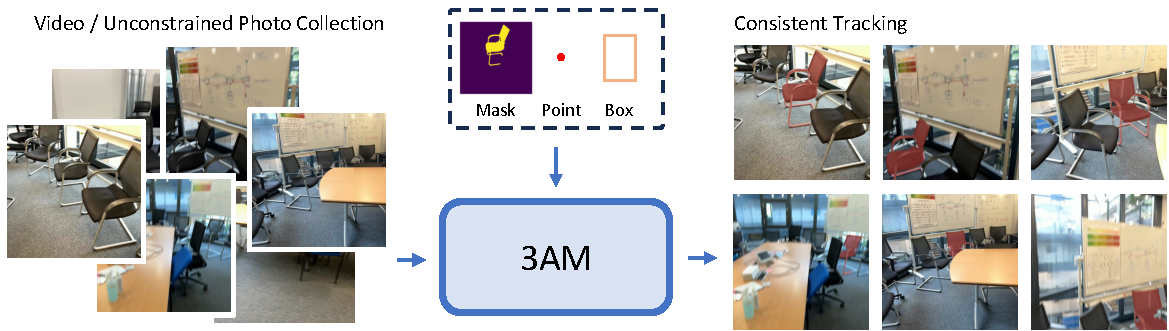
\includegraphics[width=\textwidth]{figs/teasers.pdf}
}
\vspace{-6mm}
\caption{\textbf{Overview of 3AM.}  
Given an input video or an unconstrained photo collection, 3AM takes a user-provided prompt, e.g., mask, point, or box, and produces a consistent object track across all views.  
Our method maintains cross-view correspondence even under large viewpoint changes, cluttered scenes, and variations in capture conditions, enabling robust object tracking from both videos and casual multi-view image sets.
}
\vspace{-3mm}
\label{teaser}
\end{center}

\begin{abstract}
Video object segmentation methods like SAM2 achieve strong performance through memory-based architectures but struggle under large viewpoint changes due to reliance on appearance features. Traditional 3D instance segmentation methods address viewpoint consistency but require camera poses, depth maps, and expensive preprocessing. We introduce 3AM, a training-time enhancement that integrates 3D-aware features from MUSt3R into SAM2. Our lightweight Feature Merger fuses multi-level MUSt3R features that encode implicit geometric correspondence. Combined with SAM2’s appearance features, the model achieves geometry-consistent recognition grounded in both spatial position and visual similarity. We propose a field-of-view aware sampling strategy ensuring frames observe spatially consistent object regions for reliable 3D correspondence learning. Critically, our method requires only RGB input at inference, with no camera poses or preprocessing. On challenging datasets with wide-baseline motion (ScanNet++, Replica), 3AM substantially outperforms SAM2 and extensions, achieving 90.6\% IoU and 71.7\% Tracking Recall on ScanNet++'s Selected Subset, improving over state-of-the-art VOS methods by +15.9 and +30.4 points.
Project page: \url{https://jayisaking.github.io/3AM-Page/}
\end{abstract}
\vspace{-2em}
\section{Introduction}
\label{sec:intro}
\vspace{-1em}

\begin{figure*}[t]
    \centering
\vspace{-3mm}
    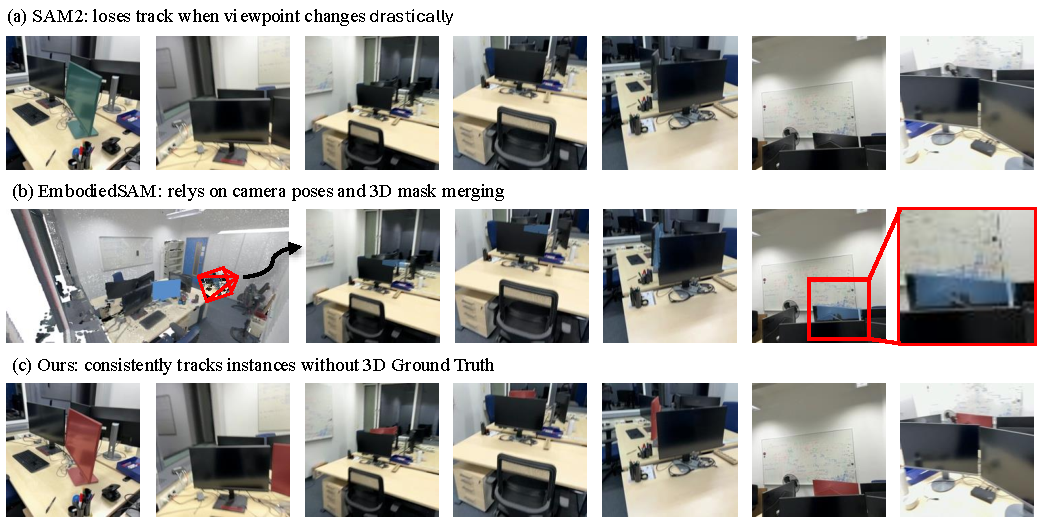
\includegraphics[width=\textwidth]{figs/comparison-teaser.pdf}
\vspace{-6mm}
    \caption{\textbf{Limitations of traditional VOS and 3D segmentation approaches, and an overview of our capability.}  
    (a) Traditional VOS methods such as SAM2~\cite{ravi2024sam2} lose track when the camera undergoes large viewpoint changes, causing masks to drift or disappear.  
    (b) 3D segmentation approaches rely on accurate camera poses and explicit 3D mask merging; they often propagate errors when the 3D reconstruction is incomplete or noisy.  
    (c) Our \textbf{3AM} consistently tracks object instances across drastic viewpoint changes without requiring camera poses or 3D ground-truth masks, demonstrating robust cross-view correspondence purely from geometry-aware 2D tracking.
    }
    \label{fig:intro-comparison}
\vspace{-3mm}
\end{figure*}

Video object segmentation (VOS) identifies and tracks target objects throughout a video sequence with consistent masks across frames. This is fundamental to autonomous driving, robotics, augmented reality, and video editing. A critical challenge is maintaining object identity under large viewpoint variations, temporary disappearances, or similar distractors. Traditional VOS methods rely on 2D appearance features and fail when the object appears dramatically different from varying viewpoints. For embodied AI in dynamic 3D environments, consistently recognizing objects across diverse viewpoints is essential for robust scene understanding.

Recent video object segmentation advances follow two parallel lines. First, 2D foundation models with memory-based architectures: SAM2~\cite{ravi2024sam2} introduced promptable segmentation with streaming memory and spatio-temporal attention. SAM2Long~\cite{ding2024sam2long} employs memory trees for long-range identity preservation, while DAM4SAM~\cite{videnovic2025distractor} incorporates distractor-aware updates. However, purely 2D approaches fail under large viewpoint changes as appearance features cannot establish reliable correspondence. Second, 3D instance segmentation methods: proposal-centric approaches like Mask3D~\cite{schult2022mask3d} and OneFormer3D~\cite{kolodiazhnyi2024oneformer3d} operate on point clouds, while projection-based methods like Open3DIS~\cite{nguyen2024open3dis}, SAM3D~\cite{yang2023sam3d}, and SAM2Object~\cite{zhao2025sam2object} lift 2D masks to 3D. These require camera poses, depth maps, preprocessing, and super-linear computational scaling.

Both paradigms have critical gaps (\cref{fig:intro-comparison}). 2D methods like SAM2 excel at efficiency but lack geometric awareness, failing under viewpoint variation (\cref{fig:intro-comparison}a). MOSEv2~\cite{ding2025mosev2} shows significant degradation under wide-baseline changes. Conversely, 3D methods achieve better consistency but require explicit 3D inputs (\cref{fig:intro-comparison}b) and struggle to generalize. 2D-to-3D lifting suffers from view-inconsistent predictions~\cite{jia2024sceneverse,peng2023openscene,takmaz2023openmask3d,xu2024embodiedsam,zhao2025sam2object}. End-to-end approaches like PanSt3R~\cite{zust2025panst3r} require offline processing. \emph{Can we achieve 3D-aware, viewpoint-robust segmentation while preserving promptability and efficiency, without explicit 3D supervision?} (\cref{fig:intro-comparison}c)

We introduce \textbf{3AM} (\cref{teaser}), a generalized 3D-aware tracker. Our key insight is that MUSt3R~\cite{cabon2025must3r} encodes implicit geometric correspondence through features learned from multi-view consistency. By fusing multi-level MUSt3R features with SAM2's appearance features via a lightweight Feature Merger, we enable geometry-consistent recognition based on spatial position, which at inference requires only RGB input and user prompts. We introduce a field-of-view aware sampling strategy ensuring frames observe spatially consistent object regions during training. On ScanNet++~\cite{yeshwanth2023scannet++} and Replica~\cite{replica19arxiv} with wide-baseline motion, 3AM achieves 90.6\% IoU and 71.7\% Positive IoU versus SAM2Long's 74.7\% and 41.3\% (+15.9 and +30.4 points).


In summary, our contributions are:
\begin{itemize}
\item \textbf{A key observation on the gap between 2D tracking and 3D consistency.}
2D tracking is fundamentally limited under large viewpoint variations. Existing 3D approaches require camera poses, depth, or 3D masks, often unavailable in practice. This motivates our geometry-aware framework, which achieves cross-view consistency without 3D supervision at inference.
\item \textbf{A 3D-aware feature integration framework} fusing geometric features from 3D reconstruction models with SAM2's appearance features, and \textbf{a field-of-view aware training strategy} ensuring geometric consistency for effective 3D correspondence learning.
\item \textbf{A generalized tracking framework} that adaptively reverts to the original SAM2 for non-rigid or highly dynamic objects, along with \textbf{extensive experimental evaluation} demonstrating consistent improvements over state-of-the-art VOS methods on challenging datasets such as ScanNet++ and Replica, especially under object reappearance and significant viewpoint changes, while retaining competitive performance on conventional VOS benchmarks.
\end{itemize}



\vspace{-1.5em}
\section{Related Work}
\label{sec:related}
\vspace{-1em}

\subsubsection{2D Video Object Segmentation.}
Video object segmentation (VOS) segments and tracks target objects across video sequences with temporally coherent masks~\cite{perazzi2016benchmark, caelles2017one, voigtlaender2019feelvos, maninis2018video, wu2025denver}. Early approaches relied on appearance propagation or optical flow but struggled with long-term consistency and occlusion~\cite{yang2019video, oh2019video, bhat2020learning}. Recent memory-based architectures leverage spatio-temporal attention and feature retrieval for improved object association~\cite{yang2021associating, cheng2022xmem, cheng2021rethinking, liu2022learning, park2022per, xu2022reliable, yang2024scalable, yang2022decoupling, li2024univs, cheng2024putting}, with subsequent work improving memory efficiency via restricted banks~\cite{zhou2024rmem}, gated linear matching~\cite{liu2025livos}, unified transformer frameworks~\cite{li2024onevos, zhang2025jointformer}, and dynamic anchor queries~\cite{zhou2024improving}. New benchmarks~\cite{hong2023lvos} and specialized settings such as panoramic video~\cite{yan2024panovos} and point-based prompting~\cite{mahadevan2024point} further broaden the evaluation landscape.

SAM2~\cite{ravi2024sam2}, a promptable model with streaming memory, achieves strong results across benchmarks. Follow-up efforts extend SAM2 with memory trees for long-range identity preservation~\cite{ding2024sam2long}, distractor-aware updates~\cite{videnovic2025distractor}, on-device efficiency~\cite{zhou2025edgetam}, text-driven understanding~\cite{cuttano2025samwise}, and other improvements~\cite{yang2024samurai, yang2025mosam, ye2025entitysam}. Concurrent work further combines SAM2 with large language models for reasoning-based segmentation~\cite{yuan2025sa2va, yan2024visa, bai2024one}. Despite these advances, large viewpoint changes, occlusion, and disappearance-reappearance events cause significant degradation~\cite{ding2025mosev2, xu2018youtube, perazzi2017davis}. Our method addresses these limitations by integrating 3D-aware representations into SAM2 for object-consistent segmentation under challenging viewpoint and appearance variations.

\vspace{-1em}
\subsubsection{3D Instance Segmentation.}
Mainstream 3D instance segmentation follows two tracks. Proposal-centric methods predict instance masks from point clouds with learned proposals~\cite{schult2022mask3d, jiang2020pointgroup, han2020occuseg, vu2022softgroup, misra2021end, sun2023superpoint, kolodiazhnyi2024oneformer3d, takmaz2023openmask3d, piekenbrinck2025opensplat3d}, with recent extensions adding promptable segmentation~\cite{zhou2024point} and fast open-vocabulary recognition~\cite{boudjoghra2025openyolo}. A complementary line lifts 2D results to 3D by projecting per-view masks and merging across views~\cite{yang2023sam3d, xu2024embodiedsam, nguyen2024open3dis, boudjoghra2024open, jung2025details, xu2023neurallift, kerr2023lerf, vora2021nesf, jiang2024open, bautista2022gaudi, hsu2025openm3d, tu2023imgeonet, li2024genrc}, employing superpoint affinity~\cite{yin2024sai3d}, zero-shot feature distillation~\cite{wang2024lift3d, engelmann2024opennerf}, hierarchical contrastive learning~\cite{ying2024omniseg3d, kim2024garfield}, and egocentric Gaussian lifting~\cite{gu2024egolifter}, but still depending on posed RGB-D for mask consolidation.

The rise of 3D Gaussian Splatting has further enabled semantic scene representations by distilling foundation-model features into Gaussians~\cite{qin2024langsplat, zhou2024feature, wu2024opengaussian, peng20243d}, assigning per-Gaussian identity encodings~\cite{ye2024gaussian, zhai2025panogs}, solving 2D-to-3D label assignment optimally~\cite{shen2024flashsplat}, and unifying lifting with segmentation end-to-end~\cite{zhu2025rethinking}. However, pure 2D promptable segmentation rarely suffices for 3D instances because cross-view consistency is not enforced, leading to view-inconsistent masks and fragmented instances~\cite{zhao2025sam2object, xu2024embodiedsam, peng2023openscene, takmaz2023openmask3d, jia2024sceneverse}. Our approach instead imposes 3D-aware self-consistency directly on video, preserving identity and geometry without 3D annotations or point-cloud mask merging.


\begin{figure*}[t]
  \centering
\vspace{-3mm}
  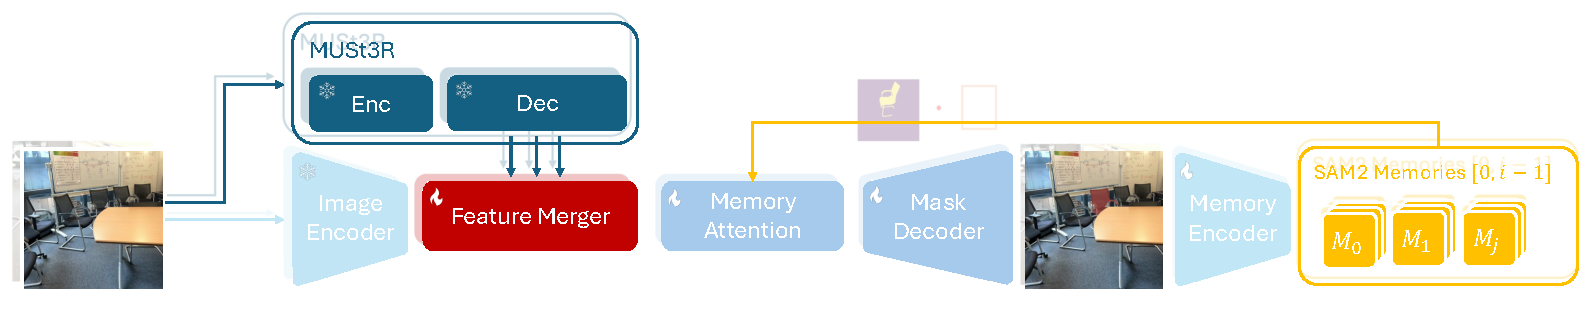
\includegraphics[width=\linewidth]{figs/pipeline.pdf}
  \vspace{-6mm}
  \caption{\textbf{3AM Pipeline Overview.} 
  Our Feature Merger fuses multi-level MUSt3R features, learned from multi-view consistency to encode implicit geometric correspondence, with SAM2's appearance features via cross-attention and convolutional refinement. These merged geometry-aware representations then undergo memory attention with previous frames and mask decoding, enabling spatially-consistent object recognition that maintains identity across large viewpoint changes without requiring camera poses at inference.
  }
  \label{fig:pipline}
\vspace{-3mm}
\end{figure*}


\vspace{-1em}
\subsubsection{End-to-End 3D-Aware Methods.}
Recent end-to-end 3D reconstruction models directly infer geometric structure from 2D inputs~\cite{cabon2025must3r, wang2024dust3r, wang2025continuous, wang2025vggt, yang2025fast3r, chen2025long3r, leroy2024grounding, wu2025point3r, charatan2024pixelsplat, ye2024no, wang20243d, lin2025longsplat, shih2025prior, fan2025spectromotion, liu2023robust, su2024boostmvsnerfs}. The DUSt3R/MASt3R family has been extended to dynamic scenes~\cite{zhang2024monst3r}, incremental reconstruction with spatial memory~\cite{wang20253d}, feed-forward Gaussian splatting~\cite{smart2024splatt3r}, efficient multi-view fusion~\cite{tang2025mv}, real-time dense SLAM~\cite{murai2025mast3r}, unconstrained structure-from-motion~\cite{duisterhof2025mast3r}, and training-free 4D reconstruction~\cite{chen2025easi3r}. Feed-forward models now also jointly predict geometry and semantics~\cite{fan2024large, sun2025uni3r, jiang2025gausstr}, with studies analyzing how different foundation models contribute complementary 3D capabilities~\cite{man2024lexicon3d}.

This progress has fueled end-to-end 3D-aware segmentation frameworks~\cite{jain2024odin, Jayanti2025SegMASt3R, li2025ovseg3r}. PanSt3R~\cite{zust2025panst3r} integrates 3D-aware features from MUSt3R~\cite{cabon2025must3r} with a transformer decoder for joint geometry and panoptic segmentation via learnable quadratic fusion. However, it is incompatible with promptable backbones (\eg, SAM2), limiting interactivity, and requires offline access to entire sequences, preventing streaming. 



% \section{Related Work}
% \label{sec:related}

% \subsubsection{2D Video Object Segmentation.}
% Video object segmentation (VOS) segments and tracks target objects across video sequences with temporally coherent masks~\cite{perazzi2016benchmark, caelles2017one, voigtlaender2019feelvos, maninis2018video, wu2025denver}. Early approaches relied on appearance propagation or optical flow but struggled with long-term consistency and occlusion~\cite{yang2019video, oh2019video, bhat2020learning}. Recent memory-based architectures leverage spatio-temporal attention and feature retrieval for improved object association~\cite{yang2021associating, cheng2022xmem, cheng2021rethinking, liu2022learning, park2022per, xu2022reliable, yang2024scalable, yang2022decoupling, li2024univs, cheng2024putting}. SAM2~\cite{ravi2024sam2}, a promptable model with streaming memory supporting points, boxes, and masks, achieves strong results across benchmarks. Follow-up efforts extend SAM2~\cite{yang2024samurai, yang2025mosam, ye2025entitysam, ding2024sam2long, videnovic2025distractor}: SAM2Long~\cite{ding2024sam2long} introduces memory trees for long-range identity preservation, while DAM4SAM~\cite{videnovic2025distractor} incorporates distractor-aware updates for cluttered scenes. Despite these advances, large viewpoint changes, occlusion, and disappearance-reappearance events cause significant degradation, as shown by MOSEv2~\cite{ding2025mosev2, xu2018youtube, perazzi2017davis}. To address these limitations, our method integrates 3D-aware representations into SAM2 for object-consistent segmentation under challenging viewpoint and appearance variations.

% \subsubsection{3D Instance Segmentation.}
% Mainstream 3D instance segmentation follows two tracks. Proposal-centric methods operate natively in 3D, predicting instance masks from point clouds with learned proposals, often requiring large-scale 3D supervision and suffering from domain shifts~\cite{schult2022mask3d, jiang2020pointgroup, han2020occuseg, vu2022softgroup, misra2021end, sun2023superpoint, kolodiazhnyi2024oneformer3d, takmaz2023openmask3d, piekenbrinck2025opensplat3d}. A complementary line lifts 2D results to 3D by projecting per-view masks and merging across views, but still depends on posed RGB-D and point clouds for mask consolidation~\cite{yang2023sam3d, xu2024embodiedsam, nguyen2024open3dis, boudjoghra2024open, jung2025details, xu2023neurallift, kerr2023lerf, vora2021nesf, jiang2024open, bautista2022gaudi, hsu2025openm3d, tu2023imgeonet, li2024genrc}. Pure 2D promptable segmentation rarely suffices for object-aligned 3D instances because cross-view association and temporal consistency are not enforced by image-space inference alone. Consequently, multi-view fusion often exhibits view-inconsistent masks, error accumulation, and fragmented 3D instances~\cite{zhao2025sam2object, xu2024embodiedsam, peng2023openscene, takmaz2023openmask3d, jia2024sceneverse}. In contrast, our approach imposes 3D-aware self-consistency directly on video, preserving identity and geometry without 3D annotations or point-cloud mask merging.


% \begin{figure*}[t]
%   \centering
%   % \vspace{-3mm}
%   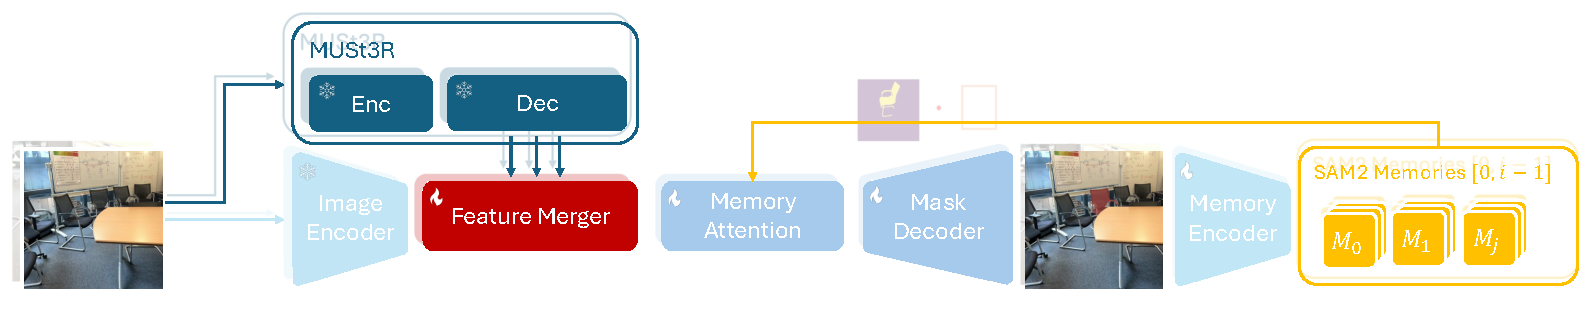
\includegraphics[width=\linewidth]{figs/pipeline.pdf}
%   \vspace{-6mm}
%   \caption{\textbf{3AM Pipeline Overview.} 
%   Our Feature Merger fuses multi-level MUSt3R features, learned from multi-view consistency to encode implicit geometric correspondence, with SAM2's appearance features via cross-attention and convolutional refinement. These merged geometry-aware representations then undergo memory attention with previous frames and mask decoding, enabling spatially-consistent object recognition that maintains identity across large viewpoint changes without requiring camera poses at inference.
%   }
%   \label{fig:pipline}
% \end{figure*}


% \subsubsection{End-to-End 3D-Aware Methods.}
% Recent progress in end-to-end 3D reconstruction shows modern models can directly infer geometric structure from 2D inputs, enhancing downstream 3D perception tasks~\cite{cabon2025must3r, wang2024dust3r, wang2025continuous, wang2025vggt, yang2025fast3r, chen2025long3r, leroy2024grounding, wu2025point3r, charatan2024pixelsplat, ye2024no, wang20243d, lin2025longsplat, shih2025prior, fan2025spectromotion, liu2023robust, su2024boostmvsnerfs}. This has fueled end-to-end 3D-aware segmentation frameworks that unify geometric reasoning and object parsing~\cite{jain2024odin, Jayanti2025SegMASt3R, li2025ovseg3r}. PanSt3R~\cite{zust2025panst3r} integrates 3D-aware features from MUSt3R~\cite{cabon2025must3r} with a transformer decoder to jointly predict geometry and panoptic segmentation, achieving multi-view consistent segmentation through learnable quadratic fusion. However, it is incompatible with promptable segmentation backbones (e.g., SAM2), limiting interactive inputs and open-vocabulary segmentation. Moreover, it requires offline access to entire image sequences, preventing online or streaming use. Our method introduces 3D-aware features into the SAM2 framework, pairing geometric consistency with promptability and broad generalization to enable object-consistent segmentation and tracking without additional 3D supervision.
\vspace{-1em}
\section{Method}
\label{sec:method}
\vspace{-0.5em}



\subsection{Problem Setting}
\vspace{-0.5em}
Given an RGB image $\mathbf{I}$ and a user-provided prompt $p$ (mask, box, or point), our goal is to identify the same object throughout a video sequence with consistent segmentation, avoiding false correspondences or identity switches across frames.
Previous approaches often fail at this goal.
\textbf{2D-based methods} (e.g., SAM2~\cite{ravi2024sam2}) rely solely on appearance features, making them sensitive to viewpoint or distance changes and prone to confusion among visually similar objects~\cite{videnovic2025distractor}, leading to frequent tracking failures over longer sequences.
\textbf{3D-based methods} (e.g., Mask3D~\cite{schult2022mask3d}, OpenYOLO3D~\cite{boudjoghra2024open}, EmbodiedSAM~\cite{xu2024esam}) localize objects using 3D mask proposals or dense 2D masks with camera poses, but require SfM or similar pipelines whose runtime and complexity grow rapidly with the number of frames, making them impractical for long sequences.
One might instead apply a 3D segmentation model on predicted geometry (e.g., point clouds from MUSt3R). However, geometry quality, especially in dynamic scenes, limits downstream segmentation reliability. Moreover, current 3D segmentation models are mainly offline, unsuitable for real-time scenarios such as robotic navigation. More importantly, large-scale training data is far more abundant in the 2D video domain, and the SAM2 model we adopt provides a strong, promptable 2D prior difficult to match with current 3D alternatives. Our method leverages this advantage by using 3D information only as a lightweight association cue rather than a hard prerequisite, maintaining a 2D segmentation framework. Specifically, we encourage geometry-consistent feature matching, enabling the model to identify the same object by recognizing its correspondence in 3D space.
% Given an RGB image $\mathbf{I}$ and a user-provided prompt $p$ (which can be a mask, box, or point), our goal is to identify the same object throughout a video sequence while maintaining consistent segmentation, i.e., avoiding false correspondences or identity switches across frames.
% Previous approaches often fail to achieve this goal. 
% \textbf{2D-based methods} (e.g., SAM2~\cite{ravi2024sam2}) rely solely on image-space appearance features, and thus are sensitive to camera viewpoint or distance changes. 
% They also struggle with visually similar or confusing objects, as partially addressed by DAM4SAM~\cite{videnovic2025distractor}, leading to frequent tracking failures as the frame sequence grows longer. 
% \textbf{3D-based methods} (e.g., Mask3D~\cite{schult2022mask3d}, OpenYOLO3D~\cite{boudjoghra2024open}, EmbodiedSAM~\cite{xu2024esam}) attempt to localize objects in space using 3D mask proposals or dense 2D masks combined with camera poses, but this requires running structure-from-motion (SfM) or similar pipelines. 
% As the number of video frames increases, both runtime and computational complexity grow rapidly, making these approaches impractical for long sequences or large scenes.
% To address these limitations, one might consider applying a 3D segmentation model on predicted geometry (e.g., point clouds from MUSt3R); however, the quality of such geometry, especially in challenging cases like dynamic scenes, significantly limits the reliability of downstream 3D segmentation. Besides, current 3D segmentation models are mainly offline, which might not be suitable for a real-time scenario, e.g., robotic navigation. More importantly, large-scale training data is far more abundant in the 2D video domain than in 3D, and the SAM2 model we adopt provides a strong, promptable 2D prior that is difficult to match with current 3D segmentation models. Our method leverages this advantage while using 3D information only as a lightweight association cue, rather than as a hard prerequisite, while maintaining a 2D segmentation framework.
% Specifically, we encourage the model to perform feature matching that is geometry-consistent, enabling it to identify the same object by recognizing its correspondence in 3D space.


\vspace{-0.5em}
\subsection{Architecture}
\vspace{-0.5em}
The overall pipeline is shown in \cref{fig:pipline}.
For each video frame $i$, our model extracts two complementary feature streams that capture appearance cues and multi-view geometric consistency. 
First, the frame is processed by the SAM2 vision encoder, producing a 2D appearance feature map $F_{\mathrm{2D}}^{i}$. 
In parallel, the same frame is passed into MUSt3R, which attends to its own multi-view memory through MUSt3R's internal cross-attention mechanism, yielding a geometry-aware feature map $F_{{3D}}^{i}$. Next, $F_{{2D}}^{i}$ and $F_{{3D}}^{i}$ are fused into a refined representation $F_{{merged}}^{i}$. The merged feature is processed by the memory attention module and the mask decoder, and is finally encoded by the memory encoder to produce memory features that will be referenced by future frames. We provide comparisons of different memory selection methods in \cref{tab:memory-selection}.


\vspace{-1em}
\subsubsection{Feature Merging.}

\begin{figure*}[t]
  \centering
\vspace{-3mm}
  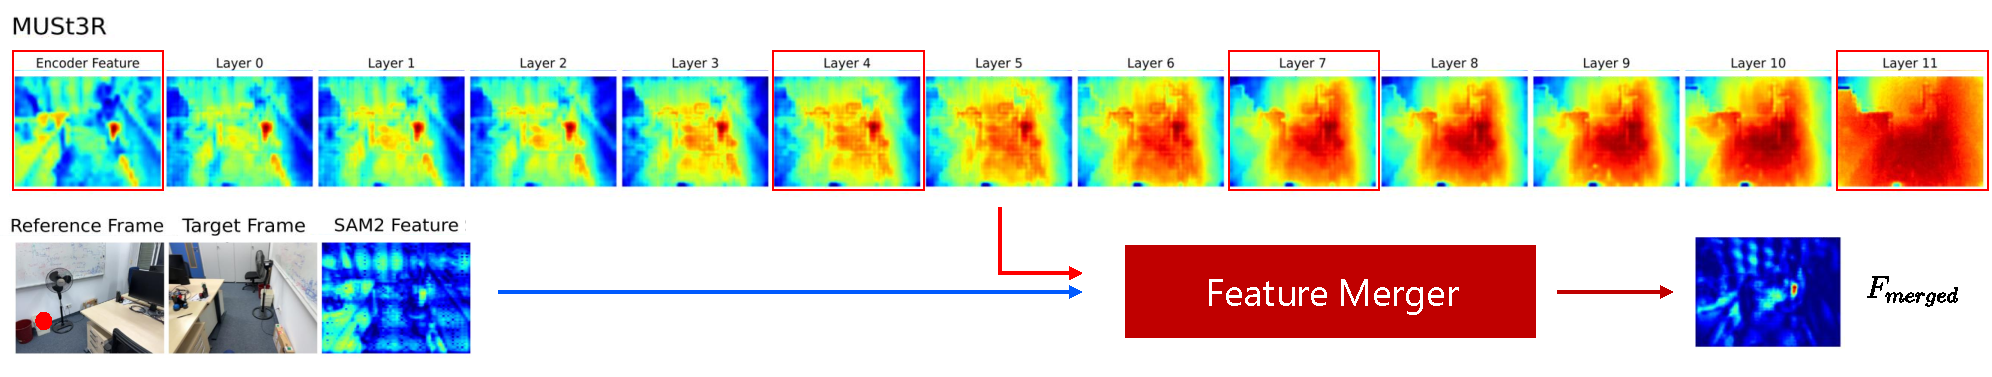
\includegraphics[width=\linewidth]{figs/FeatureMerging.pdf}
  \vspace{-6mm}
  \caption{\textbf{Illustration of Features for Feature Merging.} The heat map is computed using the cosine similarity between the red query point and the target frame. As illustrated in the lower row, vanilla SAM2 fails under large viewpoint changes. In contrast, as the MUSt3R feature hierarchy gradually shifts from semantic correspondence toward the point-cloud domain, we select intermediate layers to preserve both semantic relevance and geometric structure. By combining MUSt3R's geometric cues with SAM2's visual semantics, the merged feature $F_{{merged}}$ provides a significantly more reliable localization of the target object.
  }
  \label{fig:feature-merging}
\vspace{-3mm}
\end{figure*}

As shown in \cref{fig:feature-merging}, SAM2 becomes unreliable when the object reappears or when the viewpoint changes drastically. The heat map in the lower row demonstrates that SAM2 cannot reliably associate the query point with its target under large angular differences, revealing its limited capacity to maintain object identity when the visual appearance changes substantially.

To address this issue, we enhance SAM2 with MUSt3R features $F_{{3D}}^{i}$. The upper row of \cref{fig:feature-merging} visualizes MUSt3R activations across depth. Early layers preserve a clearer correspondence pattern with the query point, while deeper layers produce more diffuse responses. This shift reflects MUSt3R’s progression toward point-cloud decoding: the representation becomes more geometry-oriented but less semantically aligned with the 2D query. Consequently, relying solely on either early or late layers is insufficient; early layers lack explicit geometric structure, whereas late layers lose semantic clarity. We therefore sample MUSt3R features from both early and late stages to capture complementary information.

These multi-level MUSt3R features are processed by our \textbf{Feature Merger}, which jointly performs cross-attention fusion and convolutional refinement. The cross-attention blocks first integrate the sampled MUSt3R layers into a single geometry-aware feature, aligning information from different depths. 
Specifically, as shown in \cref{fig:feature-merging}, we take the MUSt3R encoder feature at the shallowest sampled depth, i.e., the most semantically rich layer, as the initial input to the Feature Merger. It first passes through a self-attention block to establish an initial semantic representation. The remaining sampled MUSt3R features are then incorporated one by one through a sequence of cross-attention layers, where the current merged representation acts as the query, and each additional MUSt3R feature provides the key–value pairs. In this way, the Feature Merger progressively integrates information from both shallow and deeper stages of MUSt3R.
The output is then fed into a convolutional stage that merges it with SAM2’s 2D feature $F_{2D}$ for restoring fine spatial detail. We further compare different 3D foundation models in \cref{tab:3D_backbone}, and more architectural details and comparisons are provided in the supplementary materials.

The final merged feature, $F_{{merged}}$, retains SAM2’s high-resolution, segmentation-aware appearance cues while incorporating MUSt3R’s geometry-aware consistency, enabling robust object localization even under severe viewpoint changes. 


% \subsubsection{Memory Selection.}
% When a new frame arrives, we cannot assume it will be as easy to segment as consecutive frames; the object may reappear after disappearance or be viewed from a drastically different angle. Therefore, it is essential to capture the object from as many viewpoints as possible. In other words, to maximize its view coverage. Following the intuition of ~\cite{cabon2025must3r}, we use MUSt3R’s output to construct a KDTree and retrieve memory frames that provide maximal viewpoint coverage for the target object.


\vspace{-0.5em}
\subsection{Training Frame Sampling}
\label{subsec:sampling}
\vspace{-0.5em}


\begin{figure*}[t]
  \centering
\vspace{-3mm}
  \begin{subfigure}{\linewidth}
    \captionsetup{justification=raggedright,singlelinecheck=false}
    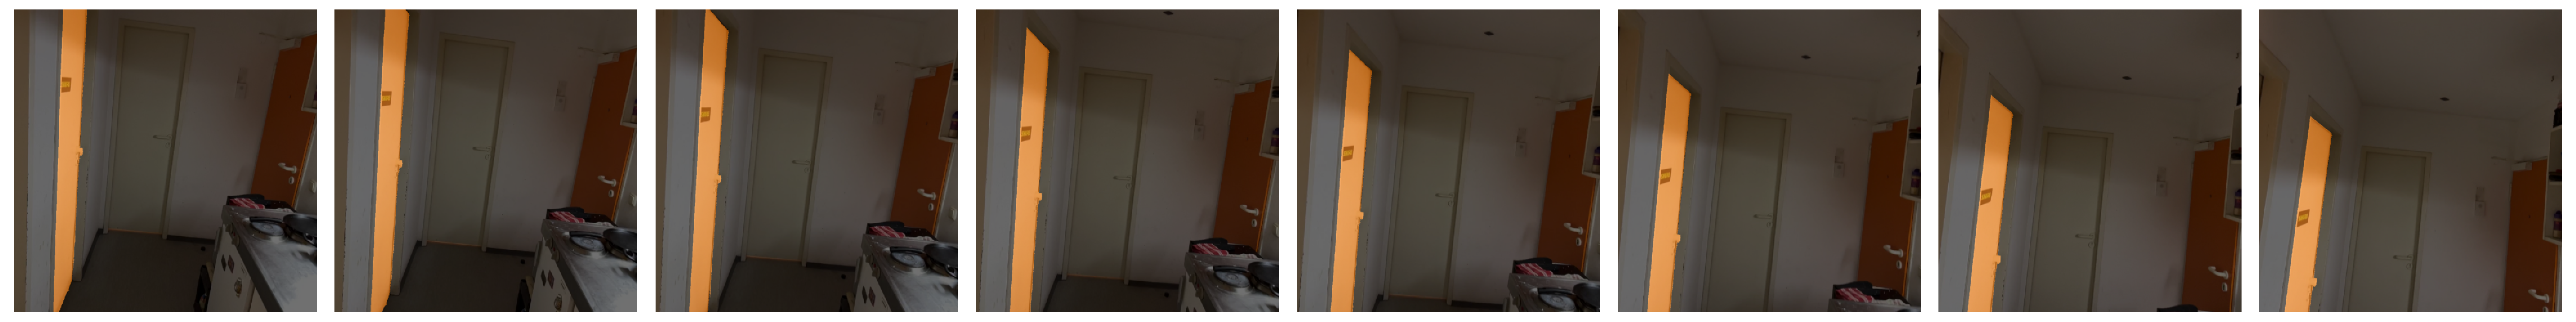
\includegraphics[width=\linewidth]{figs/scanpp_sample_continuous_sampling.pdf}
    \caption{\centering Vanilla continuous sampling strategy}
    \label{fig:cont-samp}
  \end{subfigure}
  \begin{subfigure}{\linewidth}
    \captionsetup{justification=raggedright,singlelinecheck=false}
    % \vspace{-12pt} % tighten space between caption and image
    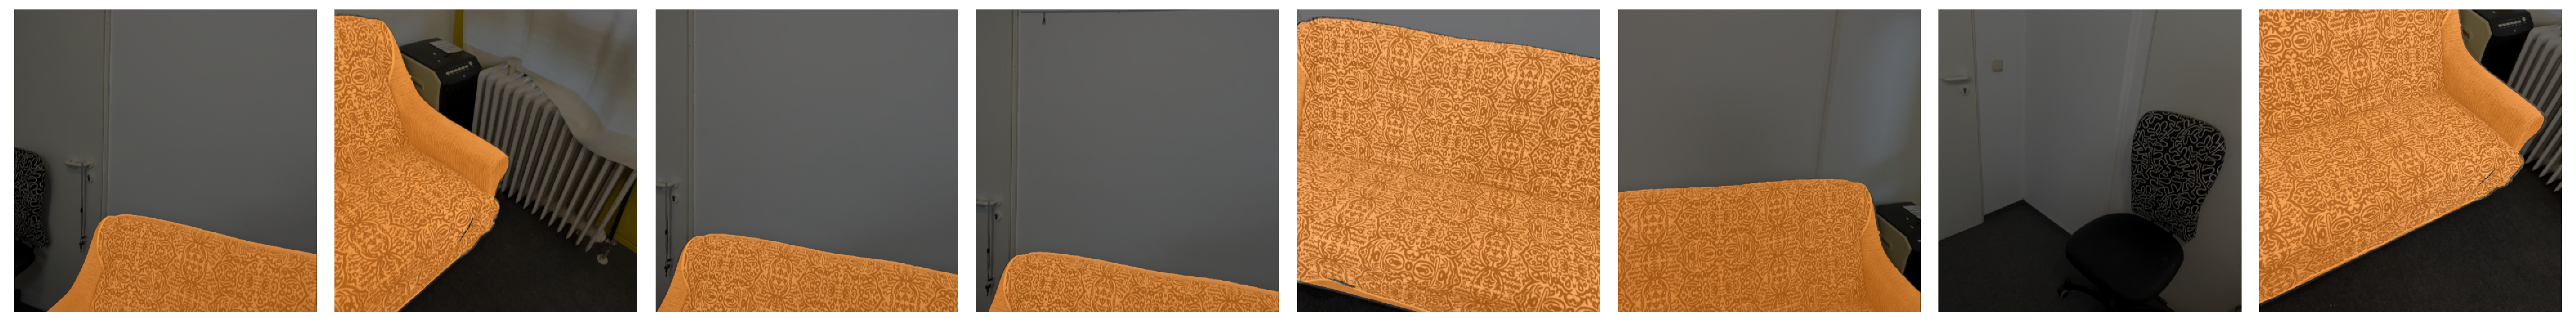
\includegraphics[width=\linewidth]{figs/scanpp_sample_no_fov_sampling.pdf}
    \caption{\centering Naive random sampling without considering field-of-view}
    \label{fig:rand-samp}
  \end{subfigure}
  \begin{subfigure}{\linewidth}
    \captionsetup{justification=raggedright,singlelinecheck=false}
    % \vspace{-12pt}
    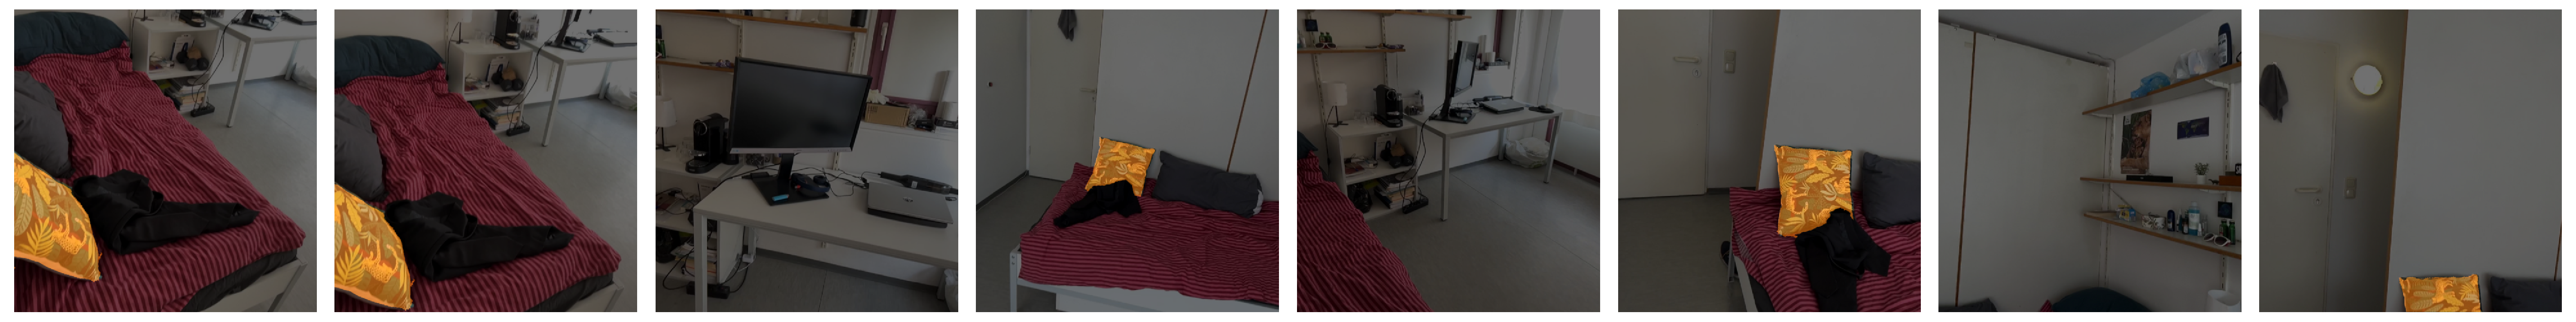
\includegraphics[width=\linewidth]{figs/scanpp_sample_fov_sampling.pdf}
    \caption{\centering Field-of-view–aware sampling strategy (Ours)}
    \label{fig:fov-samp}
  \end{subfigure}
\vspace{-6mm}
    \caption{\textbf{Overview of our sampling strategy during training.}
    (a) Continuous sampling provides densely spaced frames but offers limited viewpoint diversity.
    (b) Naïve random sampling introduces viewpoint variation but may select frames that observe spatially disjoint regions of the same object.  
    For example, frame~0 shows the left side of the couch while frame~1 shows the right side.  
    Because these regions are far apart in 3D space, treating them as the same supervisory signal forces the model to match inconsistent geometry and leads to ambiguous learning.
    (c) Our field-of-view–aware sampling retains only frames whose masked 3D points lie within the reference camera frustum over a threshold, ensuring consistent geometric overlap while preserving natural pose and occlusion variation.}

  \label{fig:pipeline}
\vspace{-3mm}
\end{figure*}


A key challenge in training our model is the limited capacity of the memory module 
(SAM2 maintains at most eight memory slots).  
To enable the model to learn robust object identification across diverse camera viewpoints, 
we must carefully design how training frames are sampled from each video sequence.

\vspace{-1em}
\subsubsection{Naïve Random Sampling.}
A straightforward strategy is to randomly sample $N$ frames from the video as in \cref{fig:rand-samp}.
This exposes the model to a broad distribution of camera viewpoints and object appearances.  
Random sampling also naturally introduces distracting or visually similar objects in the scene 
, which encourages the model to rely on 3D-aware alignment rather than purely local 2D similarity.

\vspace{-1em}
\subsubsection{Object Spanning Problem.}
However, naïve random sampling introduces a failure mode when an object occupies a large spatial extent.  
Consider a bed, table, or cabinet: two randomly sampled frames may both contain the same instance, 
yet correspond to spatially distant regions (e.g., one frame at the headboard, the other at the footboard). 
Since our objective is to enforce 3D location consistency, which is to encourage the model to identify an object by recognizing that it lies in the nearby 3D position; thus, these wide-baseline views of a large object may contradict the intended training signal.  
Although the two frames belong to the same instance, their projected 3D locations are far apart, which can confuse the learning objective.

\vspace{-1em}
\subsubsection{Field-of-View Sampling.}
For each training iteration, the first sampled frame is designated as the reference frame.  
To select the remaining $N\!-\!1$ frames, we apply a FOV-based filter using camera poses and depth.  
For every candidate frame, we back-project its object mask into 3D, transform the points into the reference frame, and re-project them onto the reference image.  
A frame is kept only if a sufficient fraction of its masked 3D points fall inside the reference camera frustum:
\[
\frac{\#\{\text{candidate masked points inside reference frustum}\}}
       {\#\{\text{masked points in candidate frame}\}}
> \tau.
\]
This ensures that selected frames observe overlapping physical regions of the object, avoiding degenerate cases where two views of the same instance correspond to distant, non-overlapping parts.  
We do not filter out partially occluded frames: frustum overlap reflects alignment in viewing direction, not full visibility, and retaining occlusion cases helps the model learn to differentiate viewpoint changes from true object absence.

Note that we apply FoV Sampling as a filter only when candidate masks contain an object. For no-object frames, which are also sampled during training, the model is simply required to predict target absence. In these cases, spatial distance does not affect the objective. That is, when views are far apart, the prediction is driven by geometric inconsistency, while for nearby views, it relies on appearance cues.

We describe our final sampling policy and its ablations in \cref{sec:exp}.

\vspace{-0.5em}
\subsection{Dynamic Object Fallback}
\vspace{-0.5em}
An intuitive limitation of our method lies in dynamic objects, whose shape, location, or orientation may change over time. Such scenarios are prevalent in traditional VOS benchmarks~\cite{perazzi2017davis, xu2018youtube, fan2019lasot}. 
Our approach relies heavily on relative appearance with respect to surrounding geometry (i.e., consistent geometrical locations across views). 
When an object undergoes significant motion, this assumption may break, potentially leading to tracking failure.
To address this issue, we detect the presence of motion using~\cite{Huang_2025_seganymotion} and revert to the original SAM2 pipeline when substantial motion is observed. 
Since the SAM2 image encoder remains frozen in our framework, we can reuse the visual feature and the additional computational overhead incurred by memory attention and mask decoder is negligible.

Empirically, we observed that dynamically toggling between 3AM and vanilla SAM2 mid-sequence (\eg, with a simple motion detection branch before mask decoder) corrupts the temporal memory bank, as the two pathways produce fundamentally different mask distributions. Therefore, we utilize a simple sequence-level fallback to the original SAM2 pipeline when substantial motion is detected. 
This design choice is grounded in a practical categorization of tracking scenarios based on the object's 
visibility with respect to the camera frustum: 
(1) \textit{Dynamic object with continuous visibility}, where the object remains within the camera frustum and 
vanilla SAM2 performs well; 
(2) \textit{Static object with temporary disappearance}, where the object leaves the camera frustum and later 
re-enters, resulting in a re-identification problem that 3AM is designed to address; and 
(3) \textit{Dynamic object with unobserved motion outside the frustum}. 

The third scenario represents an inherently ill-posed problem, as the object may move unpredictably while 
unobserved outside the camera frustum. Consequently, reliable tracking is fundamentally impossible. Since this 
extreme scenario cannot be effectively solved, engineering a complex mid-sequence fusion module is unnecessary. 
Hence a simple sequence-level switch is sufficient to cover the two tractable scenarios.
\vspace{-1em}
\section{Experiments}
\label{sec:exp}
\vspace{-1em}

\subsubsection{Training Setup.}

We train our model for 1M iterations using the AdamW optimizer with a batch size of 1, where we only set the Memory Attention, the Mask Decoder, and the Feature Merger to trainable with learning rates of 5e-6, 5e-6, and 1e-5, respectively. All loss coefficients and memory frames, which are set to 8, follow the original SAM2 configuration.

% \newcommand{\xmark}{\textcolor{red}{\large\ding{55}}}%

\vspace{-1em}
\subsubsection{Datasets.}



\begin{table}[t]
\centering
\small
\setlength{\tabcolsep}{2mm}
\vspace{-3mm}
\caption{\textbf{Datasets used for training.}
We apply FOV-aware sampling only when ground-truth geometry is available.}
\label{tab:datasets}
\vspace{-3mm}
% \resizebox{\linewidth}{!}{%
    \begin{tabular}{lccc}
    \toprule
    & ScanNet++~\cite{yeshwanth2023scannet++} & ASE~\cite{avetisyan2024scenescript} & MOSE~\cite{MOSE} \\
    \midrule
    Real                        & \ding{51} & \ding{55}          & \ding{51} \\
    Dynamic                     & \ding{55}          & \ding{55}          & \ding{51} \\
    FOV sampling prob           & 0.8        & 0.8        & 0.0 \\
    \#Scenes / Videos           & 855        & 2612        & 1453 \\
    \bottomrule
    \end{tabular}
% }
\vspace{-3mm}
\end{table}


Intuitively, to equip the model with the ability to segment objects consistently across a scene, it is necessary to train on 3D-based datasets that record long video sequences covering diverse camera viewpoints, along with corresponding segmentation masks and RGB frames. However, the 2D masks in such 3D-based datasets are often projected from point cloud segmentations, which can be degraded due to the sparsity of the point cloud and projection errors. 

To mitigate the imperfect 2D mask annotations common in 3D-based datasets, we train on a hybrid mixture of synthetic, real, and video segmentation datasets. Specifically, the Aria Synthetic Dataset(ASE)~\cite{avetisyan2024scenescript} provides clean geometric supervision, ScanNet++~\cite{yeshwanth2023scannet++} offers realistic indoor 3D consistency, and MOSE\cite{MOSE} maintains the original temporally coherent masks. This combination enables balanced spatial and temporal learning. Note that to remain consistent with our sampling strategy described in \cref{subsec:sampling}, we apply continuous sampling on MOSE, as it does not provide camera poses or depth maps.  
For ASE and ScanNet++, which include calibrated geometry, we adopt a mixed policy: continuous sampling with probability 0.2 and our FOV-aware sampling with probability 0.8.  
The FOV threshold $\tau$ is set to 0.25. To apply our sampling strategy, we first run MUSt3R inference on every scene in ScanNet++ and MOSE and store the resulting features. These precomputed features are then used during training to enable FOV-aware sampling.
For continuous sampled batches, MUSt3R is executed on the fly.  



\vspace{-0.5em}
\subsection{2D Evaluation.}
\vspace{-0.5em}

To demonstrate the capability of our model, we evaluate its performance on 2D object tracking under challenging camera motion. 
Specifically, we focus on scenarios where the camera undergoes significant translation and rotation, and where objects may disappear and later reappear.  
Traditional VOS benchmarks such as LVOS~\cite{hong2023lvos}, VOST~\cite{tokmakov2023vost}, DAVIS~\cite{perazzi2017davis}, and YTOS~\cite{xu2018youtube} primarily assume a relatively fixed camera and stable scene surroundings, making them insufficient for testing robustness under large viewpoint changes.

To address this limitation, we use 3D-based datasets, ScanNet++~\cite{yeshwanth2023scannet++} and Replica~\cite{replica19arxiv}, which naturally provide extensive camera trajectory variation due to their 3D reconstruction requirements.  
Their wide-baseline viewpoints make them suitable for evaluating consistency under severe pose changes.
For each scene in both datasets, we use ground-truth camera poses to project 3D instance masks onto the 2D frames.  
We then select the frame with the largest visible mask area as the conditioning frame and perform forward and backward tracking from that reference.

\vspace{-1em}
\subsubsection{Compared Methods.}
For comparison, we use SAM2 as the state-of-the-art VOS baseline.  
We also include the following works: SAM2Long~\cite{ding2024sam2long} and DAM4SAM~\cite{videnovic2025distractor}, which enhance SAM2 by improving its memory selection for more robust tracking. Note that our method, \textbf{3AM}, uses the naive memory mechanism of the original SAM2 in all reported results unless specified otherwise.

\vspace{-1em}
\subsubsection{Metrics.}
We use three complementary metrics to evaluate tracking quality.
\textbf{IoU} is computed over all frames, including those where the object is absent, reflecting overall stability.
\textbf{Tracking Recall} measures accuracy only on frames where a target object is present.
\textbf{Accuracy} is further restricted to visible frames where the prediction has non-zero overlap with ground truth, capturing accuracy conditioned on successful localization.
These metrics assess robustness to disappearance and accuracy when tracking succeeds.

\vspace{-1em}
\subsubsection{ScanNet++.}

\begin{table*}[t]
\centering
\small
\vspace{-3mm}
\caption{\textbf{Video Object Segmentation results on the ScanNet++ \cite{yeshwanth2023scannet++} and VOS datasets.} 
Tracking Recall is computed over frames with object presence. 
Accuracy is computed over frames where a ground-truth object exists and the IoU of prediction and GT $\neq 0$.}
\label{tab:scannetpp-2d}
  \vspace{-3mm}
\resizebox{\textwidth}{!}{
\begin{tabular}{lcccccccccccc}
\toprule
\multirow{2}{*}{Method} &
\multirow{2}{*}{FPS} &
Mem &
\multicolumn{3}{c}{ScanNet++ Whole Set} &
\multicolumn{3}{c}{ScanNet++ Selected Subset} & $\text{DAVIS}_{17}$ & LaSOT & $\text{LaSOT}_{\text{ext}}$ & DiDi \\
\cmidrule(lr){3-3}\cmidrule(lr){4-6} \cmidrule(lr){7-9} \cmidrule(lr){10-10} \cmidrule(lr){11-11} \cmidrule(lr){12-12} \cmidrule(lr){13-13}
& & G & IoU $\uparrow$ & Tracking Recall $\uparrow$ & Accuracy $\uparrow$ & IoU $\uparrow$ & {Tracking Recall} $\uparrow$ & Accuracy $\uparrow$ & J\&F $\uparrow$  & AUC $\uparrow$  & AUC $\uparrow$  & Accuracy $\uparrow$  \\
\midrule
SAM2~\cite{ravi2024sam2}  & 14.4 & 3.6 & 0.4392 & 0.0235 & 0.0831 & 0.3397 & 0.0179 & 0.0395 & 89.0 & 70.0 & 56.9 & 0.720 \\
SAM2Long~\cite{ding2024sam2long} & 7.1 & 6.8 & \cellcolor{orange!25}0.8233 & \cellcolor{yellow!25}0.4166 & \cellcolor{orange!25}0.6855 & \cellcolor{yellow!25}0.7474 & \cellcolor{yellow!25}0.4133 &  \cellcolor{yellow!25}0.6382 & 88.3 & 73.9 & - & 0.719 \\
DAM4SAM~\cite{videnovic2025distractor} & 12.3 & 3.5 & \cellcolor{yellow!25}0.8205 & \cellcolor{orange!25}0.4193 & \cellcolor{yellow!25}0.6783 & \cellcolor{orange!25}0.7648 & \cellcolor{orange!25}0.4356 & \cellcolor{orange!25}0.6650 & 86.6 & 75.1 & 60.9 & 0.727\\
3AM & 6.3 & 3.6 & \cellcolor{red!25}0.8898 & \cellcolor{red!25}0.5630 & \cellcolor{red!25}0.7155 & \cellcolor{red!25}0.9061 & \cellcolor{red!25}0.7168 & \cellcolor{red!25}0.7737 & 89.0 & 70.0 & 56.9 & 0.720 \\
\bottomrule
\end{tabular}
}
\vspace{-3mm}
\end{table*}

\begin{figure*}[t]
    \centering
     % \vspace{-3mm}
    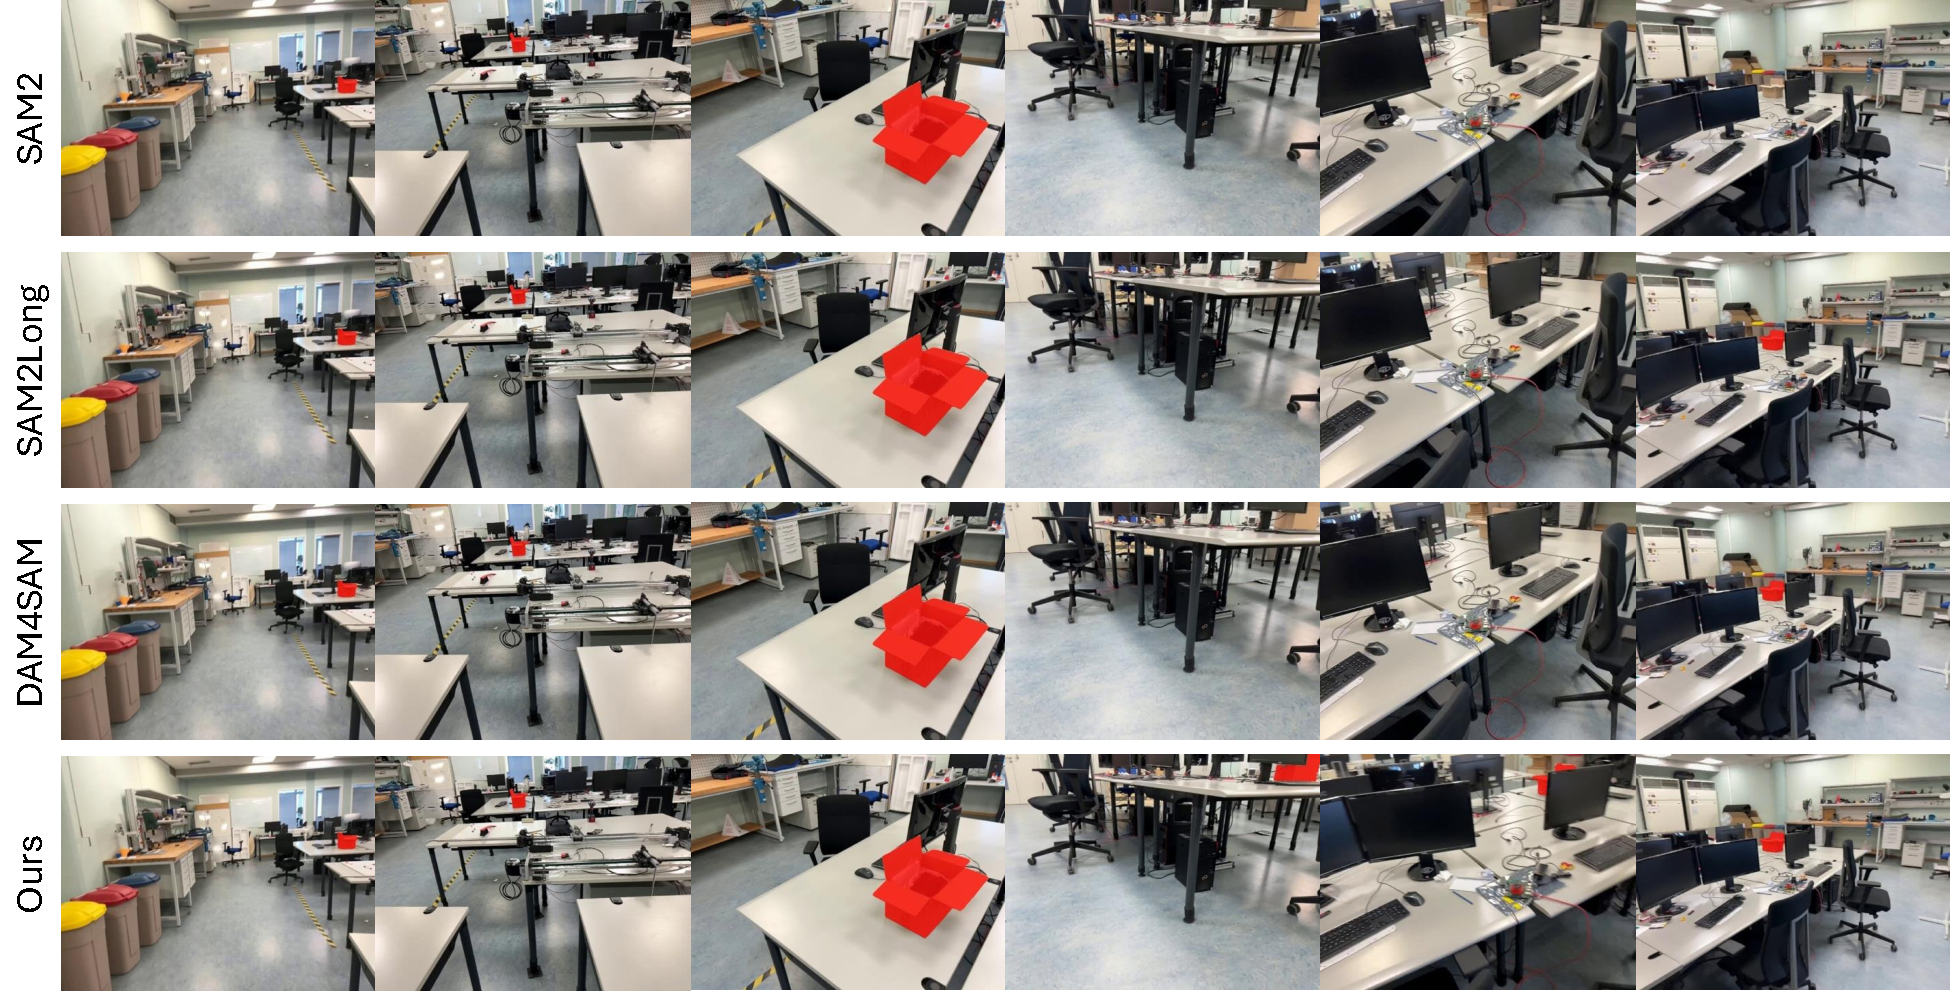
\includegraphics[width=1.0\textwidth]{figs/vis_comp.pdf}
    \vspace{-6mm}
    \caption{
    \textbf{Visual comparison of VOS methods.} The leftmost frame is used as the conditioned frame and provides the reference mask.
    }
    \label{fig:vis_comp}
\end{figure*}

The results are shown in \cref{tab:scannetpp-2d}, and we provide visualization at \cref{fig:vis_comp}.
On the ScanNet++ dataset, we further evaluate performance on a \emph{Selected Subset} specifically constructed to emphasize object reappearance.  
For each object track, we count the number of non-continuous visible segments, 
where a segment is defined as any contiguous span of visible frames whose length $\ell$ exceeds a minimal threshold $\ell_{\min}$.
Objects with frequent reappearance are typically associated with large viewpoint changes, since each disappearance–reappearance cycle often corresponds to observing the object from a substantially different angle or position.  
This subset, therefore, provides a focused evaluation of robustness under severe pose variation.

3AM achieves the best performance on both the \emph{Whole Set} (IoU 0.8898, highest Recall and Accuracy) and the challenging \emph{Selected Subset} (IoU 0.9061, Recall 0.7168, Accuracy 0.7737), highlighting its ability to maintain object identity even when the object reappears under large changes in viewpoint and spatial configuration. With a simple fallback mechanism, it also retains competitive results on conventional VOS benchmarks~\cite{perazzi2017davis, fan2019lasot, videnovic2025distractor} as shown in \cref{tab:scannetpp-2d}.

\vspace{-1em}
\subsubsection{Two-view Matching Comparison with SegMASt3R.}
We further compare our 3AM with SegMASt3R~\cite{Jayanti2025SegMASt3R}, a two-view matching approach built on MASt3R that associates segment masks between two images under large viewpoint changes, in \cref{tab:two_view_comparison}. SegMASt3R is not directly prompable and does not natively support $>2$ multiview tracking. Nevertheless, we include it as a strong two-view baseline by adopting the following protocol: we use the ground-truth initial mask as the source-frame candidate, and for each subsequent frame, we independently perform two-view mask matching against the source frame. To fairly compare the two approaches, when tracking with our 3AM, we don't use any memory other than the source frame.

Under this protocol, 3AM achieves \textbf{IoU} of $0.8915$, \textbf{Tracking Recall} of $0.5115$, and \textbf{Accuracy} of $0.6405$, whereas SegMASt3R obtains $0.6800$, $0.3628$, and $0.4053$, respectively. These results demonstrate 3AM not only provides stronger functionality, but also outperforms SegMASt3R even when restricted to two-view matching.

\begin{table}[t]
\centering
\setlength{\tabcolsep}{2mm}
\vspace{-3mm}
\begin{minipage}{0.48\textwidth}
\centering
\caption{{Quantitative comparison of two-view matching between 3AM and SegMASt3R on ScanNet++ Whole Set.}}
\label{tab:two_view_comparison}
\vspace{-3mm}
\resizebox{\textwidth}{!}{
\begin{tabular}{lccc}
\toprule
Method & IoU $\uparrow$ & {Tracking Recall} $\uparrow$ & Accuracy $\uparrow$\\
\midrule
SegMASt3R~\cite{Jayanti2025SegMASt3R} & 0.6800 & 0.3628 & 0.4053 \\
\rowcolor{black!10}
3AM (Ours) & \textbf{0.8915} & \textbf{0.5115} & \textbf{0.6405} \\
\bottomrule
\end{tabular}
}
\end{minipage}
\begin{minipage}{0.48\textwidth}

\centering
\caption{{Video Object Segmentation results on the Replica\cite{replica19arxiv} dataset.}}
\label{tab:replica-3d}
\vspace{-3mm}
\resizebox{\textwidth}{!}{
\begin{tabular}{lccc}
\toprule
Method & IoU $\uparrow$ & Tracking Recall $\uparrow$ & Accuracy $\uparrow$ \\
\midrule
SAM2~\cite{ravi2024sam2} & 0.4424 & 0.1432 & 0.2188 \\
SAM2Long~\cite{ding2024sam2long} & \cellcolor{yellow!25}0.7691 & \cellcolor{orange!25}0.5195 & \cellcolor{orange!25}0.6273 \\
DAM4SAM~\cite{videnovic2025distractor} & \cellcolor{orange!25}0.7744 & \cellcolor{yellow!25}0.5135 & \cellcolor{yellow!25}0.6124 \\
3AM (Ours) & \cellcolor{red!25}0.8119 & \cellcolor{red!25}0.6381 &  \cellcolor{red!25}0.6793 \\
\bottomrule
\end{tabular}
}
\end{minipage}

\vspace{-3mm}
\end{table}


\vspace{-1em}
\subsubsection{Replica.}

On the Replica dataset, 3AM achieves the best performance across all metrics (\cref{tab:replica-3d}), reaching an IoU of 0.8119 and surpassing SAM2 (0.4424), SAM2Long (0.7691), and DAM4SAM (0.7744). It also attains the highest Tracking Recall (0.6381) and Accuracy (0.6793), demonstrating robust tracking under the large viewpoint variations characteristic of Replica.

These results demonstrate that 3AM consistently surpasses prior methods and is particularly effective in scenarios involving object reappearance and large viewpoint variation, despite not relying on the explicit memory-selection mechanisms used in previous approaches. Due to space limitations, more visualization is provided in the supplementary materials.


\vspace{-0.5em}
\subsection{3D Evaluation}
\vspace{-0.5em}

We next evaluate our method on a 3D task.  
We adopt the class-agnostic 3D instance segmentation setting of ScanNet200, as it directly reflects a model’s ability to produce object-consistent predictions in 3D scenes.  
Prior approaches typically require explicit 3D fusion\cite{xu2024esam} or merging\cite{yang2023sam3d}, regardless of whether the proposals originate from 2D masks\cite{jung2025details} or 3D detectors\cite{boudjoghra2025openyolo, nguyen2024open3dis}.
Our goal is to demonstrate that this additional 3D-space merging is unnecessary: if 2D tracking is geometrically consistent across views, then reliable 3D instances can be obtained simply by projecting the tracked 2D masks into 3D.

Concretely, we follow prior methods\cite{zhao2025sam2object} and generate 2D proposals from SAM2 on keyframes selected by a stride-based sampling.  
These proposals are then propagated with 3AM, whose improved cross-view consistency enables stable object identification across multiple camera viewpoints.  
We perform merging using IoU and inter-mask precision to associate proposals over time, and project the resulting 2D tracks into 3D.  
In contrast, previous SAM2-based methods\cite{zhao2025sam2object} rely heavily on 3D merging because their tracking often drifts or fails under large viewpoint changes.  
Further implementation details are provided in the supplementary material.

As shown in Table~\ref{tab:scannet200-class-agnostic}, 3AM achieves the highest performance among online methods, with an AP of 47.3 and strong AP$_{50}$ and AP$_{25}$ scores (59.7 and 75.3).    
These results highlight a central finding of our work: robust 3D instance segmentation can emerge from geometry-aware tracking without heavy 3D supervision.



\begin{table}[t]
\centering
\small
\setlength{\tabcolsep}{2mm}
\vspace{-3mm}
\caption{\textbf{Class-agnostic 3D instance segmentation results of different methods on ScanNet200 dataset.}}
\label{tab:scannet200-class-agnostic}
\vspace{-3mm}
% \resizebox{\columnwidth}{!}{
\begin{tabular}{lccccc}
\toprule
Method & Type & 3D GT & AP $\uparrow$ & AP$_{50}$ $\uparrow$ & AP$_{25}$ $\uparrow$ \\
\midrule
SAMPro3D~\cite{xu2025sampro3d} & Offline & Yes & 18.0 & 32.8 & 56.1 \\
Open3DIS~\cite{nguyen2024open3dis} & Offline & Yes & \cellcolor{yellow!25}34.6 & 43.1 & 48.5 \\
SAI3D~\cite{yin2024sai3d} & Offline & Yes & 28.2 & 47.2 & 67.9 \\
SAM2Object~\cite{zhao2025sam2object} & Offline & Yes & 34.0 & \cellcolor{yellow!25}52.7 & \cellcolor{yellow!25}70.3 \\
\midrule
SAM3D~\cite{yang2023sam3d} & Online & Yes & 20.2 & 35.7 & 55.5 \\
ESAM~\cite{xu2024esam} & Online & Yes & \cellcolor{orange!25}42.2 & \cellcolor{red!25}63.7 & \cellcolor{red!25}79.6 \\
\midrule
3AM (Ours) & Online & No & \cellcolor{red!25}47.3 & \cellcolor{orange!25}59.7 & \cellcolor{orange!25}75.3 \\
\bottomrule
\end{tabular}
% }
\vspace{-3mm}
\end{table}


\vspace{-0.5em}
\subsection{Ablation Study}
\vspace{-0.5em}

\subsubsection{Component Analysis.}
We provide ablation studies in \cref{tab:component-eval} for Feature Source, Feature Merger Architecture, and Sampling Strategy.
We evaluate variants using MUSt3R or SAM2 features alone under the same training protocol to demonstrate that both features are necessary. MUSt3R provides geometric grounding, while SAM2 captures appearance correspondence. Without MUSt3R, relying solely on appearance matching from SAM2 introduces ambiguity and leads to degraded performance. One thing to note is that SAM2 performs worse after finetuning. We attribute this degradation to the absence of grounding information from MUSt3R, which causes the memory attention to be mistrained due to insufficient reference cues for distinguishing different objects.
Regarding the sampling strategy, naively applying random sampling results in worse performance than continuous sampling. When valid masks exist in both views, enforcing associations across large spatial discrepancies introduces ambiguity and leads to slower convergence.

\begin{table*}[t]
\centering
\setlength{\tabcolsep}{2mm}
\caption{\textbf{Component analysis on ScanNet++ selected subset.}}
\label{tab:component-eval}
\vspace{-3mm}
\resizebox{\textwidth}{!}{%
\begin{tabular}{cccccc}
\toprule
Feature Source & Feature Merger & Sampling Strategy & IoU & Tracking Recall & Accuracy \\
\midrule
SAM2 \& MUSt3R & Addition \& Convolution & FoV Sampling & 0.8771 & 0.6481 & 0.7149\\
SAM2 \& MUSt3R & Concatentation \& Attention & FoV Sampling & 0.8831 & 0.6744 & 0.7462\\
SAM2 \& MUSt3R & Hierarchical Cross Attention (Final) & Continuous Sampling & 0.7925 & 0.6518 & 0.7513\\
SAM2 \& MUSt3R & Hierarchical Cross Attention (Final) & Random Sampling & 0.7363 & 0.5371 & 0.6311 \\
MUSt3R  & - & FoV Sampling & 0.8461 & 0.5471 & 0.4129 \\
SAM2 & - & FoV Sampling & 0.6628 & 0.0038 & 0.0276 \\
SAM2 \& MUSt3R & Hierarchical Cross Attention (Final) & FoV Sampling & 0.9061 & 0.7168 & 0.7737\\
\bottomrule
\end{tabular}
}
% \vspace{-3mm}
\end{table*}

\vspace{-1em}
\subsubsection{Memory Selection.}
\label{subsubsec-memory-select}

\begin{table}[t]
\centering
\small
\setlength{\tabcolsep}{2mm}
\vspace{-3mm}

\begin{minipage}{0.48\textwidth}
\caption{Comparison of different memory selection methods on ScanNet++ Whole Set.}
\label{tab:memory-selection}
\vspace{-3mm}
\resizebox{\textwidth}{!}{
\begin{tabular}{lccc}
\toprule
Method & IoU $\uparrow$ & Tracking Recall $\uparrow$ & Accuracy $\uparrow$ \\
\midrule
3AM & \cellcolor{yellow!25}0.8898 & \cellcolor{yellow!25}0.5630 & \cellcolor{yellow!25}0.7155 \\
DAM4SAM-3AM~\cite{videnovic2025distractor} & \cellcolor{orange!25}0.8941 & \cellcolor{orange!25}0.5471 &  \cellcolor{orange!25}0.7204 \\
SAM2Long-3AM~\cite{ding2024sam2long} & \cellcolor{red!25}0.9004 & \cellcolor{red!25}0.5498 & \cellcolor{red!25}0.7361 \\
\bottomrule
\end{tabular}
}
\end{minipage}
\begin{minipage}{0.48\textwidth}
\caption{Comparison of different 3D reconstruction backbones.}
\label{tab:3D_backbone}
\resizebox{\textwidth}{!}{
\begin{tabular}{lccc}
\toprule
\textbf{Model} & \textbf{Online} & \textbf{Frame Num} & \textbf{ScanNet++ Selected Subset Tracking Recall} \\
\midrule
VGGT & $\times$ & $\sim$200       & --      \\
$\pi^3$ & $\times$ & $\sim$300    & --      \\
CUT3R & \checkmark & $>10{,}000$  &  0.2751 \\
\rowcolor{black!10}
MUSt3R & \checkmark & $>10{,}000$  &  \textbf{0.7168}  \\
\bottomrule
\end{tabular}
}
\end{minipage}
\vspace{-3mm}
\end{table}

We further analyze the role of memory selection by combining 3AM with existing strategies proposed for SAM2.  
Table~\ref{tab:memory-selection} reports results on the ScanNet++ Whole Set.  
3AM, which uses the original SAM2 memory-selection mechanism, already achieves strong performance with an IoU of 0.8898.  
When we incorporate alternative memory-selection policies, such as those from DAM4SAM~\cite{videnovic2025distractor} or SAM2Long~\cite{ding2024sam2long}, we observe modest improvements: DAM4SAM-3AM slightly increases Accuracy to 0.7204, while SAM2Long-3AM achieves the highest IoU (0.9004) and Accuracy (0.7361).
These results suggest that 3AM already delivers strong and stable performance without relying on specialized memory-selection policies.  
While alternative strategies such as those from SAM2Long or DAM4SAM offer small additional gains, their impact is relatively limited compared to the improvements brought by 3AM itself.  
We view the design of memory-selection mechanisms tailored specifically for 3AM as an interesting direction for future work.

\vspace{-1em}
\subsubsection{3D Foundataion Models.}
\label{subsubsec-3d-models}

\begin{figure}[t]
    \centering
    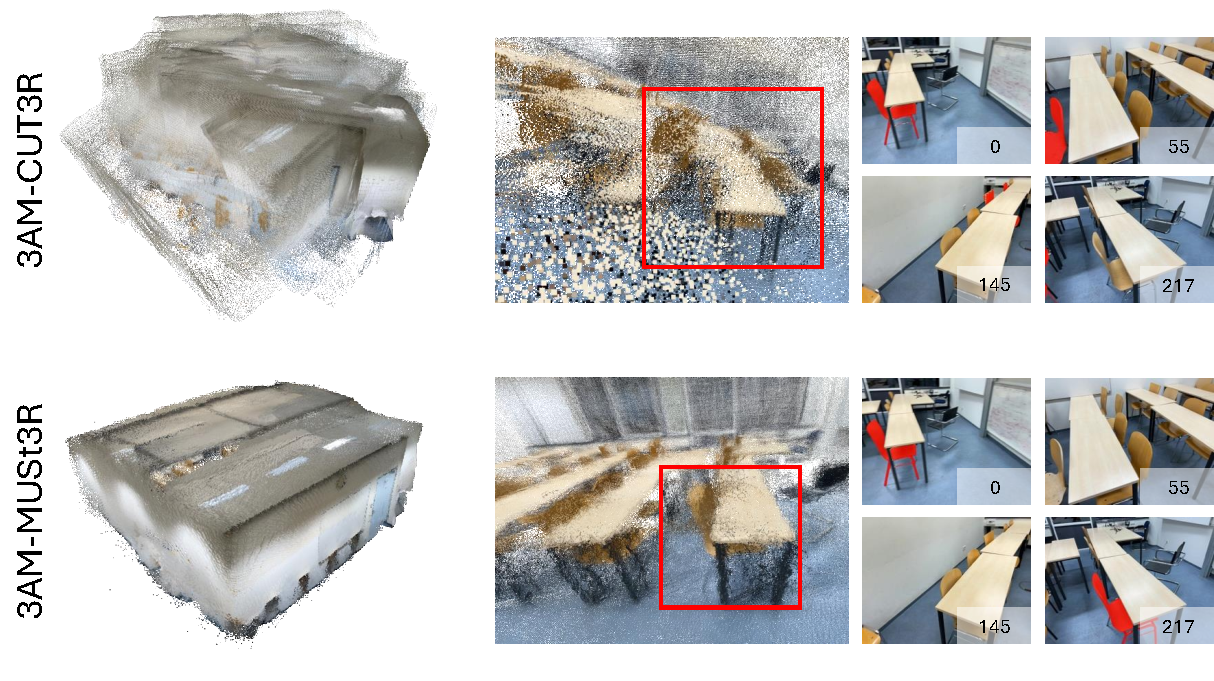
\includegraphics[width=1.0\linewidth]{figs/vis_cut3r.pdf}
    \vspace{-6mm}
    \caption{
    \textbf{Visual comparison of different 3D reconstruction backbones.} (\emph{Top}) CUT3R's reconstruction lacks stable object alignment; the same table appears at inconsistent 3D locations. Such geometric instability weakens feature distinctiveness, making reliable tracking difficult. (\emph{Bottom}) In contrast, MUSt3R provides coherent and stable object alignment across viewpoints, yielding features that preserve object identity and enable robust tracking
    % \textbf{Visual comparison of different 3D reconstruction backbones used for feature extraction.}  
    % The top row shows the geometry produced by CUT3R, whose reconstruction lacks stable object alignment, i.e., the same table appears at inconsistent 3D locations.  
    % Since our method relies on backbone features to establish cross-view correspondence, such geometric instability weakens the distinctiveness and consistency of the extracted features, making reliable tracking difficult.  
    % In contrast, MUSt3R (bottom row) provides much more coherent and stable object alignment across viewpoints, yielding feature representations that preserve object identity under large pose changes and enabling significantly more robust tracking.
    }
    \label{fig:comp_3r}
\end{figure}

We compare 3D foundation models in Table~\ref{tab:3D_backbone}. VGGT and $\pi^3$ operate offline on frame batches, unsuitable for online tracking. CUT3R supports online operation, but yields limited instance-level alignment as shown in \cref{fig:comp_3r}, reflected by its Tracking Recall of 0.2751 on the ScanNet++ Selected Subset. MUSt3R is fully online with substantially stronger object alignment across viewpoints. This alignment is essential: consistent 3D alignment enables stable 2D cross-view correspondence, allowing reliable mask propagation without explicit 3D merging.

% To understand the impact of different 3D reconstruction backbones, we compare several recent 3D foundation models in Table~\ref{tab:3D_backbone}.  
% VGGT and $\pi^3$ are offline models that operate on frame batches and therefore cannot be used in an online tracking pipeline.  
% CUT3R supports online operation but yields limited instance-level alignment as shown in \cref{fig:comp_3r}, reflected by its Tracking Recall of 0.2751 on the ScanNet++ Selected Subset.
% In contrast, MUSt3R is fully online and produces substantially stronger object-level alignment across viewpoints.  
% We argue that such alignment is essential for our task: consistent alignment in 3D directly supports stable cross-view correspondence in 2D, enabling reliable mask propagation without the need for explicit 3D-space merging.

% More ablation studies are provided in the supplementary materials.
\vspace{-1em}
\section{Conclusion}
\label{sec:conclusion}
\vspace{-1em}
We introduce 3AM, integrating 3D-aware features into SAM2 for viewpoint-robust video object segmentation. Through our Feature Merger and field-of-view aware sampling, 3AM achieves geometry-consistent tracking requiring only RGB at inference. On wide-baseline datasets, 3AM substantially outperforms state-of-the-art VOS methods, achieving gains of +15.9 and +30.4 points on the ScanNet++ Selected Subset, while automatically switching back to SAM2's capability to handle dynamic video scenarios.

% We introduce 3AM, a training-time enhancement to SAM2 that integrates 3D-aware features for viewpoint-robust video object segmentation. By fusing multi-level MUSt3R features with SAM2's appearance features, our method enables geometry-consistent recognition based on spatial position. Our field-of-view aware sampling ensures effective 3D correspondence learning. 3AM requires only RGB input at inference, with no camera poses or preprocessing. On challenging datasets with wide-baseline camera motion (ScanNet++, Replica), 3AM substantially outperforms SAM2 and its extensions, achieving +15.9 and +30.4 point improvements over SAM2Long on ScanNet++'s Selected Subset. 3AM bridges 2D promptable segmentation and 3D geometric awareness for robust video object segmentation.

% \paragraph{Limitations.}
% Our method is constrained by object visibility. When objects move outside the camera's field of view, tracking fails due to missing observations.

% Like most VOS-based approaches, our method is constrained by the visibility of the target object.  
% If the object undergoes large motion outside the camera’s field of view, for example, chairs being moved behind the camera, no visual evidence is available for the model to maintain identity.  
% In such cases, tracking is fundamentally limited by missing observations.


% \par\vfill\par
% References should start immediately after the main text, but can continue past p.\ 14 if needed. 
% \clearpage  % TODO FINAL: This \clearpage needs to be removed from both review and camera-ready versions.

\section*{Acknowledgements}
This work was supported by NVIDIA Taiwan AI Research \& Development Center (TRDC). This research was funded by the National Science and Technology Council, Taiwan, under Grants NSTC 112-2222-E-A49-004-MY2 and 113-2628-E-A49-023-. Yu-Lun Liu acknowledges the Yushan Young Fellow Program by the MOE in Taiwan.

% ---- Bibliography ----
%
% BibTeX users should specify bibliography style 'splncs04'.
% References will then be sorted and formatted in the correct style.
%
\bibliographystyle{splncs04}
\bibliography{main}



\clearpage
\appendix
\section{Overview}
\label{sec:appendix_overview}
This supplementary material presents additional results to complement the main manuscript. 
First, we provide all the implementation details, including network architectures in~\cref{sec:details}.
Next, we elaborate on training details, such as the FoV sampling and datasets in~\cref{sec:training_details}.
Then, we describe how we perform class-agnostic instance segmentation in~\cref{sec:class_agnostic}.
Finally, we provide more qualitative comparisons on both video object tracking and class-agnostic instance segmentation in~\cref{sec:more_qualitative}.
% In addition to this document, we provide an interactive HTML interface to compare our video results with state-of-the-art methods.
In addition to this document, we provide additional video results to compare with state-of-the-art methods.


\section{Implementation Details} \label{sec:details}
Through all experiments, we use SAM~2.1-Large as our baseline due to computational resource constraints. A Hiera~\cite{ryali2023hiera} image encoder produces multi-scale features, where stride-16 and stride-32 outputs (Stages 3/4) are fused via an FPN~\cite{lin2017featureFPN} with convolutions to obtain frame embeddings, while shallow features (stride 4/8) from Stages 1/2 are injected only into the mask decoder to recover fine boundaries. Memory attention uses sinusoidal absolute positional embeddings together with 2D RoPE; object pointer tokens do not use RoPE, and we adopt $L=4$ layers. The prompt encoder follows SAM, and the mask decoder uses the mask token as the object pointer stored in the memory bank. An additional token predicts object visibility via an MLP head, and occluded frames receive a learned occlusion embedding in memory. As in SAM~2, the decoder outputs multiple mask candidates and selects the one with the highest predicted IoU when ambiguity persists. The memory encoder reuses Hiera features without a separate backbone; memory features are projected to 64 dimensions, and the 256-dim pointer is split into four 64-d tokens for cross-attention. For multi-object videos, the image encoder is shared while each object maintains an independent memory bank and decoder.
 
\subsection{Feature Merger}

% As illustrated in \cref{fig:feature-merging}, we use multi-layer feature from must3r decoder. 
% Note that we maintain MUSt3R's memory as it is, i.e. we do that alter the memory selection mechanism in MUSt3R, which is essentirally select by maximizing view coverage. The $[\text{encoder feature},4,7,11]$ layer index is selected empirically, as we want to introduce both semantic-aware(from early layers) and geometry-aware(from late layers, as it decodes point clouds from linear layer after the final transformer layer in must3r decoder, and we will also use the output point cloud).  After selecting the must3r features, we next merge it the cross attention layers. Specifically, we first gatther the positional embedding to following merging. The positional embedding is obtained by passing through the point map and ray map from must3r output, and we call this PE3D. PE2D is obtained by using Must3r's positional embedding. During merging, We first pass encoder feature through a conv layer to reduce dim from 1024 to 768, add PE3D, and then pass through a self attention layer with PE2D, which is called $F_{coarse}$. For the following $i\in [4, 7, 11]$, we update the $F_{coarse}$ by Attention layers, i.e. $F_{coarse}=FFN(CrossAttn(SelfAttn(F_{coarse}+PE3D), F_i+PE3D)$. We omit the normalization and skip connection for simplicity. After these attention blocks, we next pass $F_{coarse}$ through interplation and convolution layers and then concatenate with $F_{2D}$ from the SAM Image encoder, which is then refined by a convolution block to align the feature dims with $F_{2D}$. The final feature $F_{merged}$ is used as main feature for memory attention and memory encoding. Note that the shallow featrues from Hiera from Stages 1/2 are left untouched so that we can use such visual feature for fine mask output in mask decoder.

As illustrated in \cref{fig:feature-merging}, our method uses multi-layer features from the MUSt3R decoder.  
We keep MUSt3R’s memory mechanism unchanged—i.e., we do not modify its view-coverage–based memory selection.  
We empirically select the layer indices $[\text{encoder}, 4, 7, 11]$ to incorporate both semantic cues from early layers and geometry-aware signals from later layers, as deeper decoder layers in MUSt3R increasingly capture 3D structure and directly decode point clouds.

After selecting the MUSt3R features, we merge them using a sequence of cross-attention operations.  
We first construct positional embeddings: PE3D is obtained by processing the point map and ray map produced by MUSt3R, while PE2D is taken from MUSt3R’s 2D positional encoding.  
The encoder feature is projected from 1024 to 768 channels using a $1\!\times\!1$ convolution, added with PE3D, and then passed through a self-attention layer with PE2D to form an initial coarse feature $F_{\text{coarse}}$.

For each selected MUSt3R layer $F_i$ with $i \in \{4,7,11\}$, we update $F_{\text{coarse}}$ using:
\begin{equation} \small
\resizebox{\columnwidth}{!}{$
F_{\text{coarse}}
\leftarrow
\mathrm{FFN}\!\left(
\mathrm{CrossAttn}\!\big(
\mathrm{SelfAttn}(F_{\text{coarse}} + \mathrm{PE3D}),
\, F_i + \mathrm{PE3D}
\big)\right).
$}
\end{equation}
We omit normalization and skip connections for clarity.

After the attention fusion, $F_{\text{coarse}}$ is upsampled and refined by a $3\!\times\!3$ convolution, then concatenated with the Hiera image-encoder feature $F_{2D}$ from SAM~2, followed by an additional convolution block to match the feature dimensions.  
The resulting feature $F_{\text{merged}}$ is used for memory attention and memory encoding.  
We leave the shallow Hiera features from Stages~1 and~2 untouched so that the mask decoder can still rely on strong low-level visual cues for producing high-resolution segmentation outputs.


\section{Training Details} \label{sec:training_details}
\subsection{Field-of-View Sampling}
We do not use 100\% FOV-aware sampling because we observe that applying FOV filtering to every batch degrades the model’s original feature-matching ability inherited from SAM2.  
When all training samples come from drastically different viewpoints, the model is over-regularized toward cross-view matching and loses its within-view correspondence skills, leading to a form of feature collapse.  
% We therefore mix FOV-aware and continuous sampling, and analyze different sampling ratios in \cref{tab:sampling-ratio}.



% \begin{table}[t]
% \centering
% \caption{\textbf{Video Object Segmentation results between different sampling ratio on ScanNet++ Selected Set.} 
% Positive IoU is computed over frames with ground-truth masks. 
% Successful IoU is computed over frames where a ground-truth object exists and the IoU of prediction and GT $\neq 0$.}
% \label{tab:sampling-ratio}
% \resizebox{\columnwidth}{!}{
% \begin{tabular}{lccc}
% \toprule
% Method / FoV-aware Sampling Prob. & IoU $\uparrow$ & Positive IoU $\uparrow$ & Successful IoU $\uparrow$ \\
% \midrule
% Vanilla SAM2 / - & 0.3397 & 0.0179 & 0.0395 \\
% 3AM / 0.0 & 0.6945 & 0.4781 & 0.5024 \\
% 3AM / 0.8 & 0.9061 & 0.7168 & 0.7737 \\
% 3AM / 1.0 & 0.5811 & 0.3576 & 0.3913 \\
% \bottomrule
% \end{tabular}
% }
% \end{table}
\subsection{Settings}

\paragraph{Loss}
We follow SAM2's loss design without modification.  
Specifically, mask prediction is supervised using a weighted combination of focal loss (20) and dice loss (1);  
the IoU head is trained with an $\ell_{1}$ loss (1);  
and the occlusion prediction head uses a cross-entropy loss (1).

\paragraph{Prompts}
Due to the degraded 2D mask and the large viewpoint variations introduced by the sampling strategy during training, we restrict the input modality to masks only for ScanNet++ and ASE. For MOSE, we enable all prompt types, including point, box, and mask inputs.

\subsection{Datasets}
\paragraph{Aria Synthetic Environments (ASE)~\cite{avetisyan2024scenescript}}
ASE is a large-scale synthetic dataset of 100,000 procedurally generated indoor scenes rendered with simulated Aria-glass sensors. Each scene contains realistic 3D object layouts, simulated trajectories, and aligned 2D/3D annotations.
ASE enables large-scale training of 3D scene understanding, object detection, and tracking, particularly in data-hungry settings where real-world labelled data is scarce. 
We sample a total of 2{,}612 scenes whose number of views falls within a practical range:  
scenes with too few views do not provide sufficient viewpoint variation for training,  
while scenes with excessively many views lead to memory overflow when running MUSt3R. 

\paragraph{MOSE~\cite{MOSE}}
The MOSE dataset (Complex Video Object Segmentation) targets video-object segmentation in cluttered and occluded real-world scenes. It comprises 2,149 video clips with 5,200 objects from 36 categories and 431,725 high-quality masks.  
Unlike previous VOS benchmarks that feature large, salient, isolated targets, MOSE features heavy occlusion, object disappearance and re-appearance, and small/inconspicuous objects.
MOSE is primarily used to preserve the core VOS capability of our model.  
While our geometric integration encourages strong cross-view consistency, we do not want the model to over-rely on geometry and ``hallucinate'' object tracks without sufficient visual evidence; MOSE helps anchor the model to appearance-driven cues.  

Although MUSt3R supports dynamic scenes, we find that training on highly dynamic and diverse datasets such as SA-V Train leads to instability in practice. MOSE provides a more controlled level of motion and scene variation, allowing us to maintain stable learning while still leveraging dynamic-object supervision.


\paragraph{ScanNet++~\cite{yeshwanth2023scannet++}}
ScanNet++ is a high-quality indoor RGB--D reconstruction dataset that provides accurate camera poses, dense trajectories, and detailed geometric annotations.  
The public release contains over 1{,}000 reconstructed scenes, representing an expanded version of the initial smaller release\cite{yeshwanth2023scannet++}.  
Its combination of reliable geometry and viewpoint diversity makes it well suited for studying
view-consistent object tracking under large camera motions.
However, the 2D masks in ScanNet++ are generated by projecting 3D point-cloud instance labels into the image plane, which inevitably introduces reprojection noise from depth and pose inaccuracies. Besides, the pose annotations in ScanNet++ often omit long stretches of consecutive frames, as the SfM pipeline discards uncertain frames. Under such conditions, our FoV-based sampling becomes even more important.
Despite this, ScanNet++ remains valuable because it provides realistic indoor scenes with rich geometric structure and large viewpoint variation.  
Together with the other two datasets, which supply clean, frame-aligned 2D masks, this forms a complementary training combination that balances realistic geometry with high-quality appearance supervision.



\section{Class-Agnostic Instance Segmentation} \label{sec:class_agnostic}

For class-agnostic 3D instance segmentation, we proceed as follows.  
Given a set of keyframes, either sampled at a fixed interval or selected using a view-coverage criterion, we first generate 2D instance masks using SAM2’s automatic mask generator.  
For each keyframe $i$, we then propagate its instance masks forward to all subsequent frames using our model; no backward tracking is performed.
The propagated masks are lifted into 3D by back-projecting their pixels using the depth map and camera pose.  
A practical issue is the presence of reprojection errors near object boundaries, caused by depth noise and view-dependent misalignment.  
To mitigate this, we (1) compute a reprojection score using the agreement between projected depth and ground-truth depth, and (2) erode the 2D masks slightly before projection, which reduces artifacts concentrated near object edges.

After obtaining the per-frame 3D fragments, we merge them into consolidated 3D instances.  
Two scores are computed for every fragment:  
(1) a 3D overlap score in the point-cloud domain, and  
(2) a 2D temporal-overlap score based on the propagated masks along the video.  
Because our model maintains consistent object identity across the video, an object visible earlier will be recognized again whenever it reappears, providing reliable temporal evidence for merging.

Finally, after merging, duplicate assignments are resolved by majority voting at the superpoint level: each superpoint is assigned to the instance in which it is observed the greatest number of times. 





\begin{figure*}[t]
    \centering
    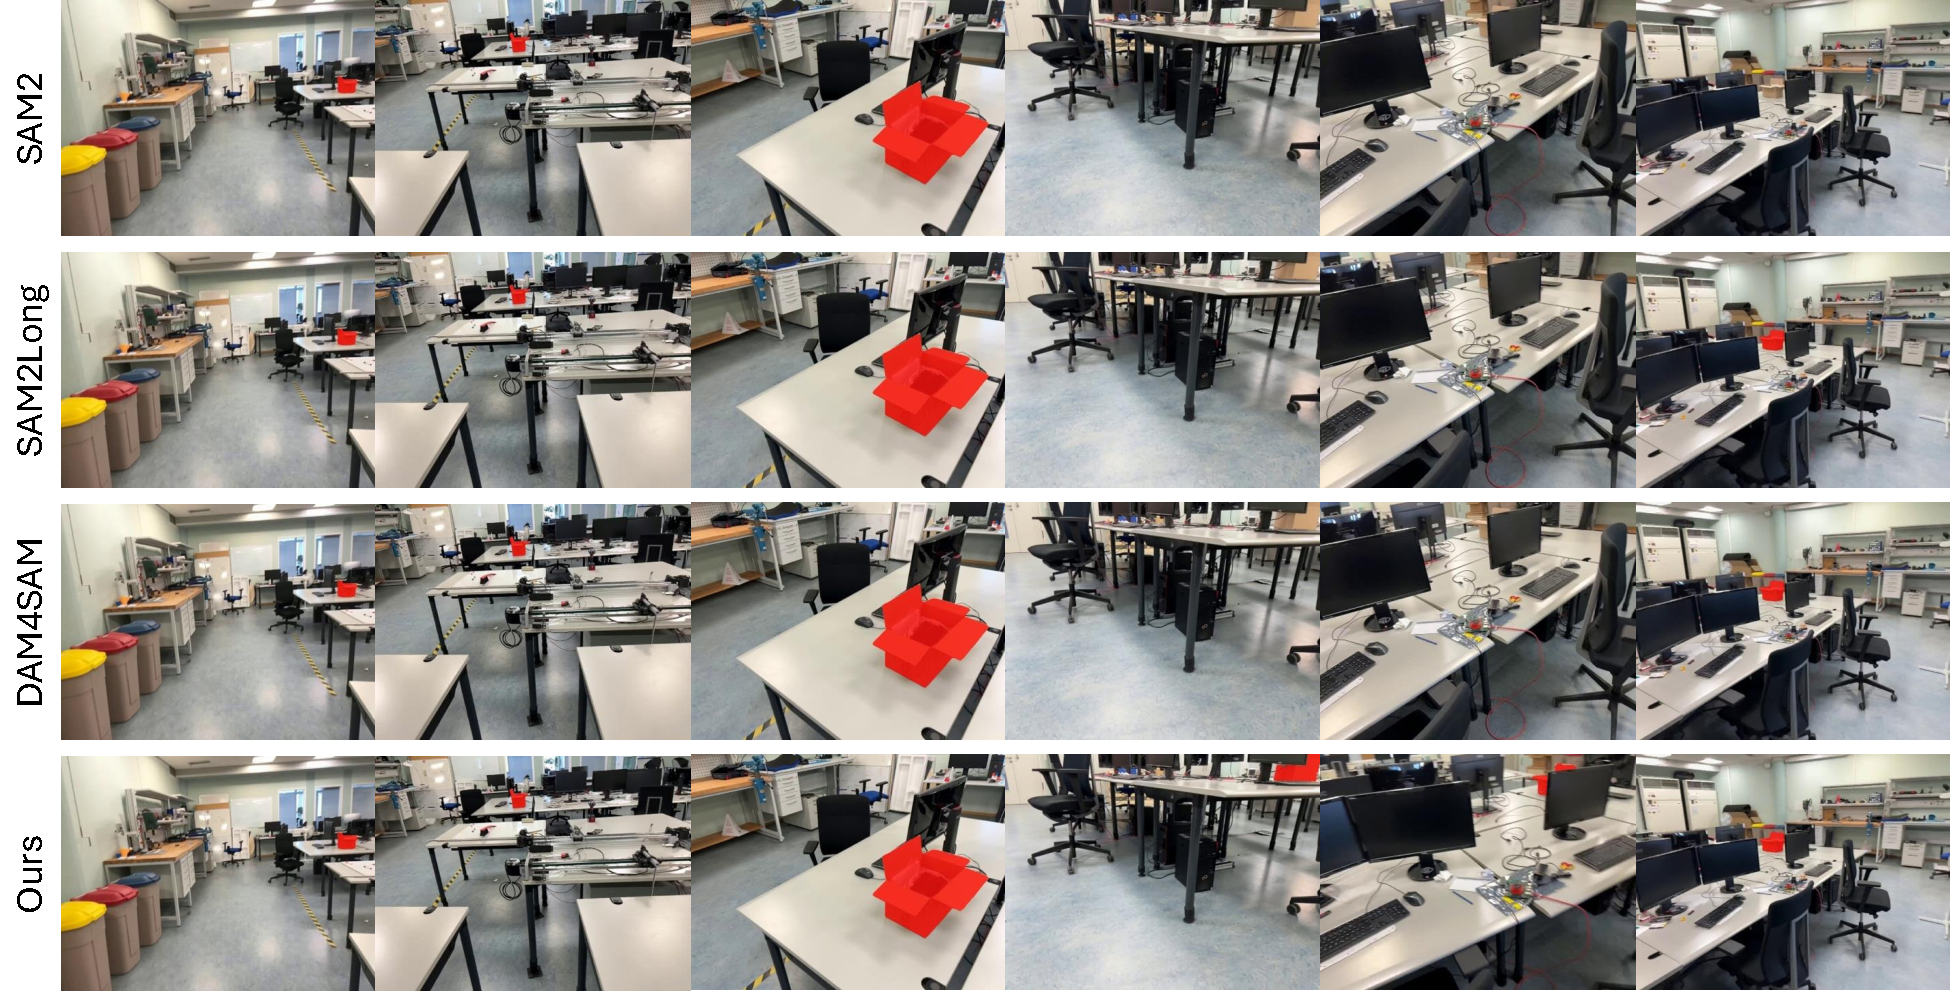
\includegraphics[width=1.0\textwidth]{figs/vis_comp.pdf}
    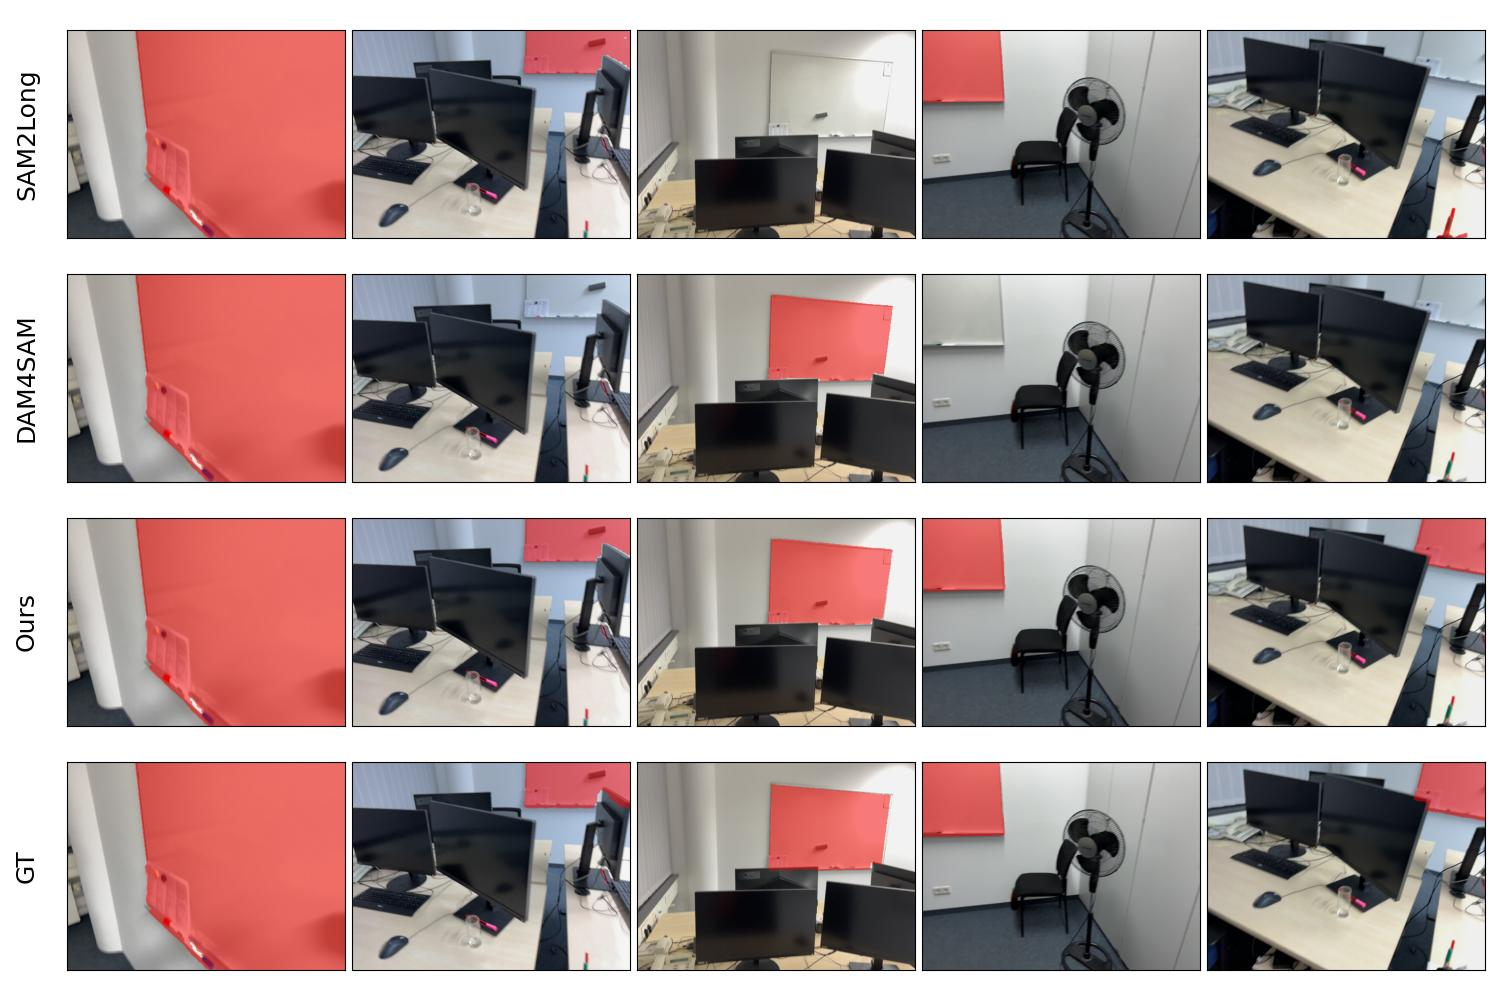
\includegraphics[width=1.0\textwidth]{figs/fig-vis/1ada7a0617/pred_masks_instance_512_7.jpg}
    \caption{
    \textbf{Visual comparison of different VOS methods}
    }
    \label{fig:vis_comp}
\end{figure*}

\begin{figure*}[t]
    \centering
    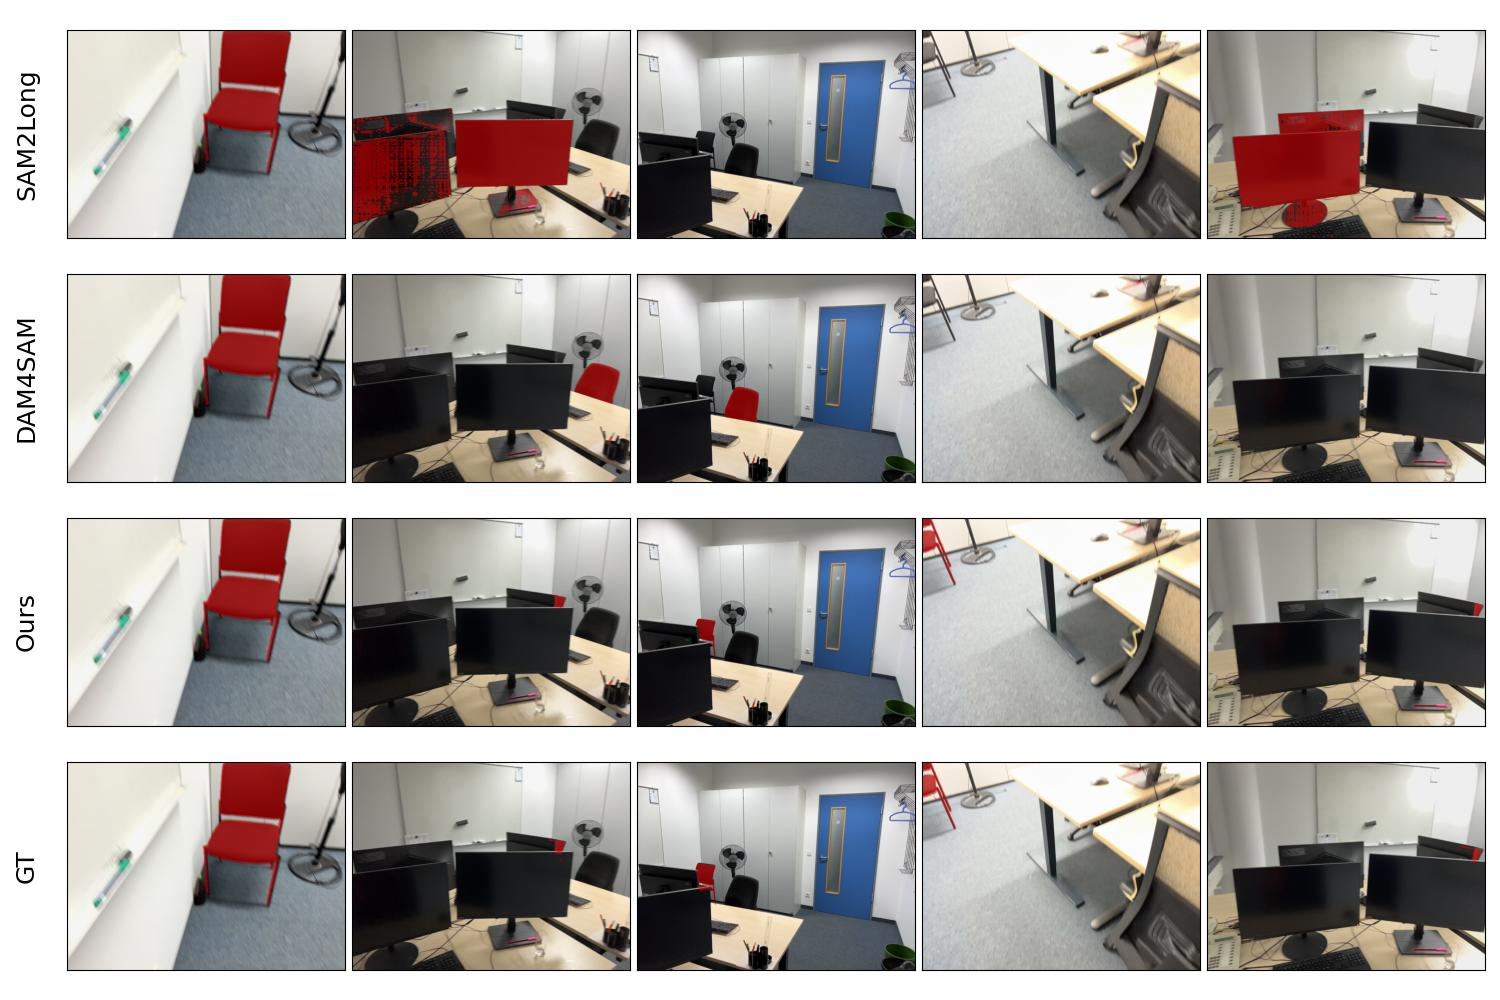
\includegraphics[width=1.0\textwidth]{figs/fig-vis/1ada7a0617/pred_masks_instance_512_11.jpg}
    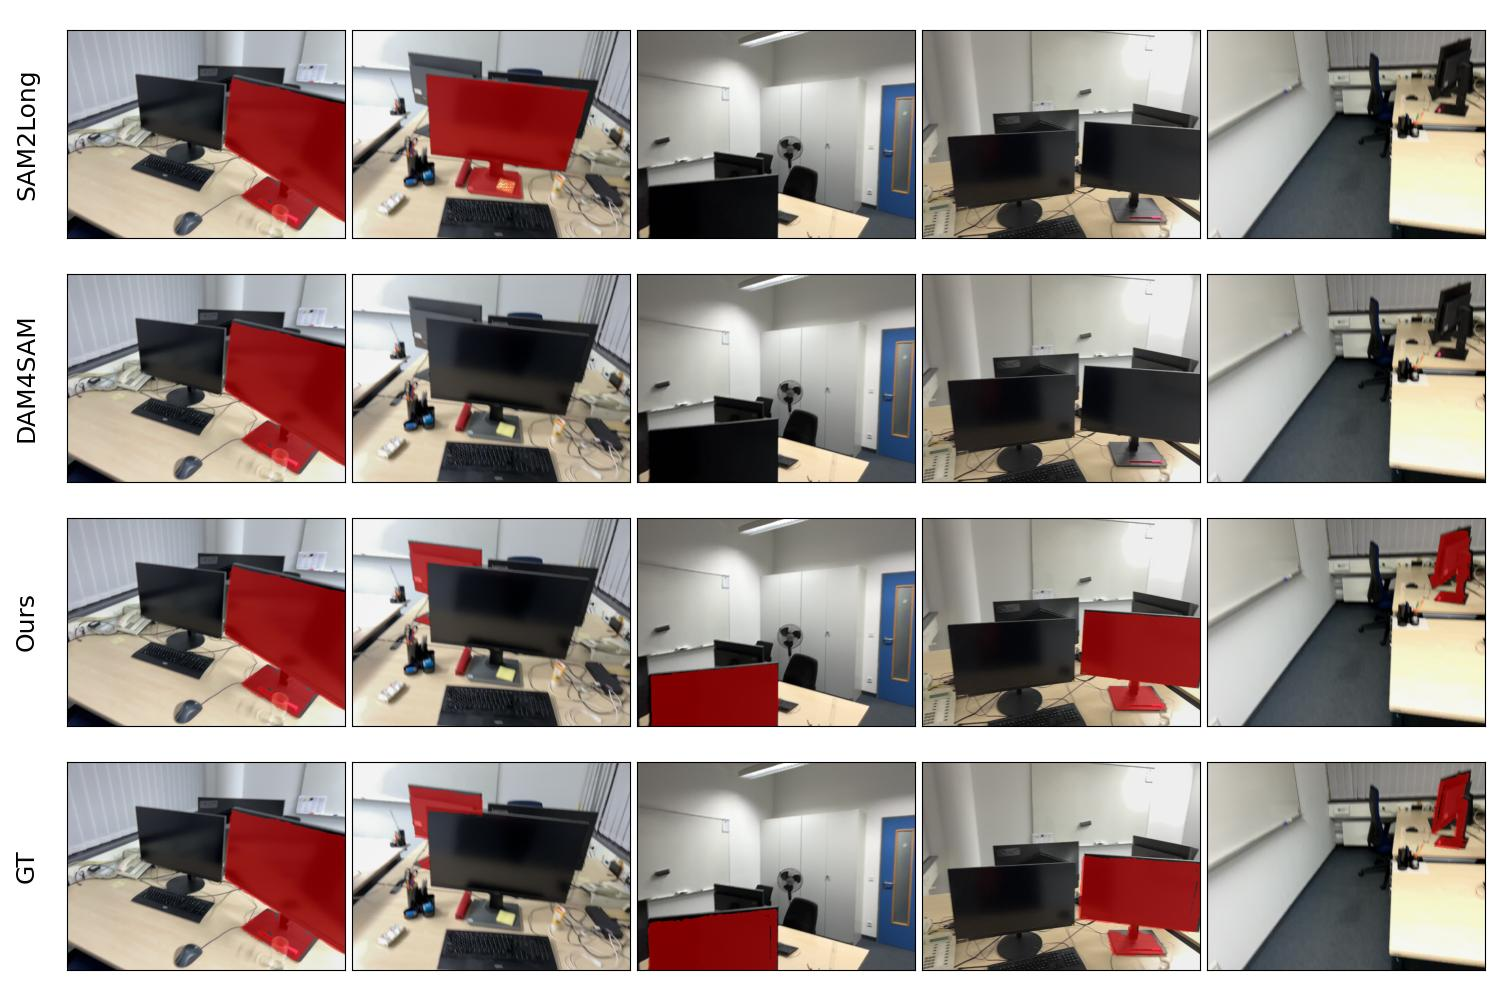
\includegraphics[width=1.0\textwidth]{figs/fig-vis/1ada7a0617/pred_masks_instance_512_36.jpg}
    \caption{
    \textbf{Visual comparison of different VOS methods}
    }
    \label{fig:vis_comp2}
\end{figure*}

\begin{figure*}[t]
    \centering
    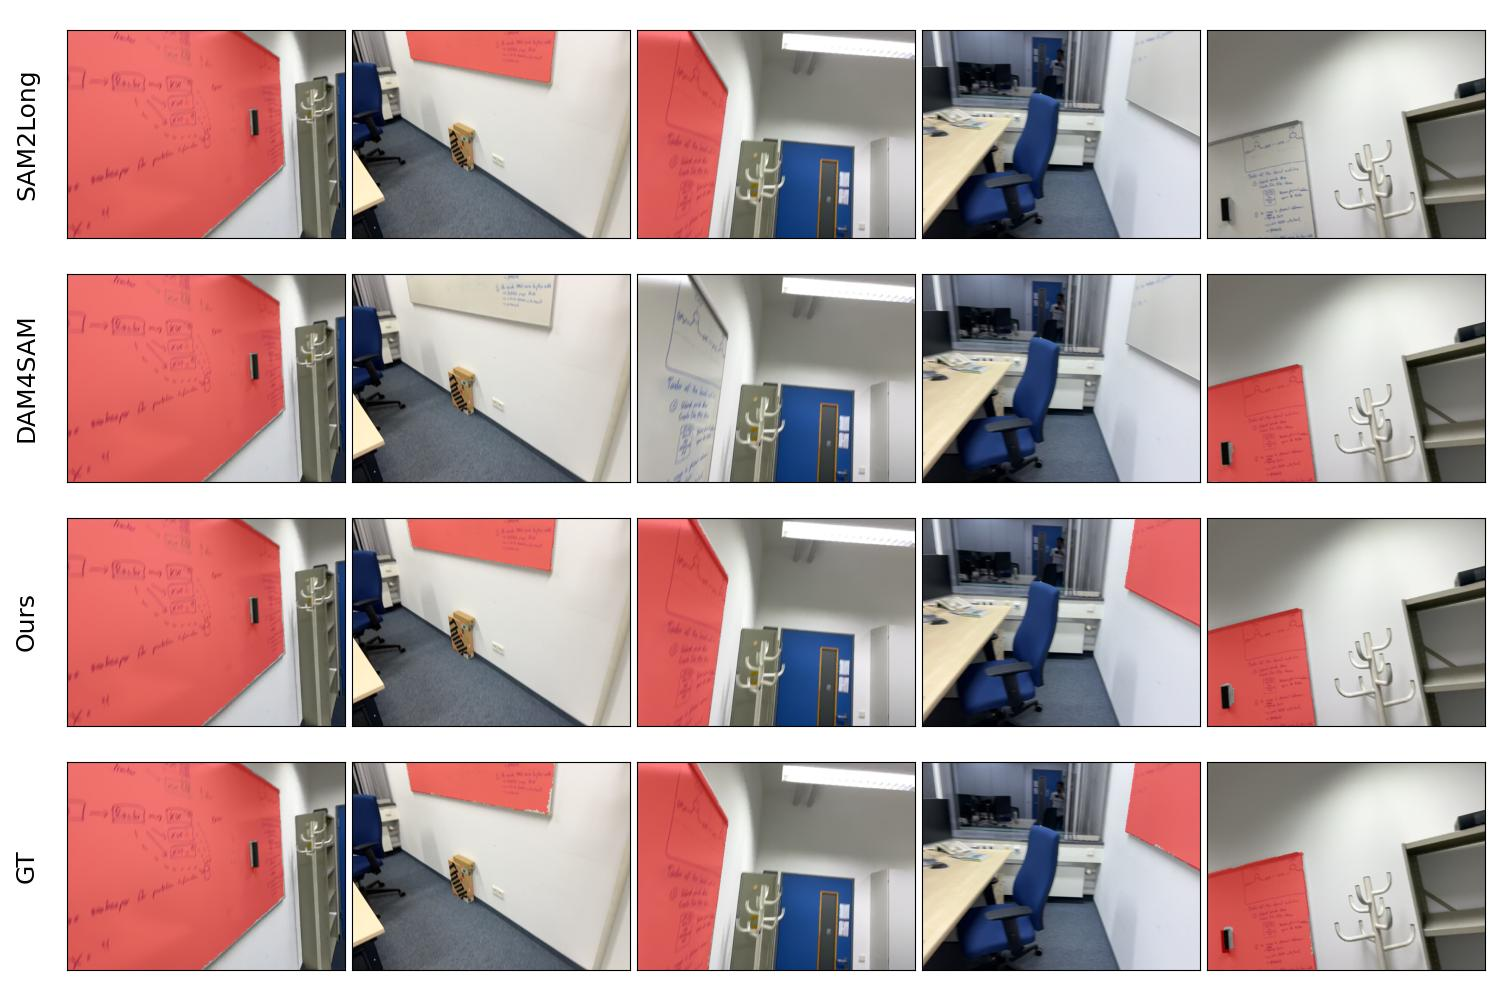
\includegraphics[width=1.0\textwidth]{figs/fig-vis/7b6477cb95/pred_masks_instance_512_10.jpg}
    
\includegraphics[width=1.0\textwidth]{figs/fig-vis/7b6477cb95/pred_masks_instance_512_11.jpg}
    \caption{
    \textbf{Visual comparison of different VOS methods}
    }
    \label{fig:vis_comp3}
\end{figure*}

\begin{figure*}[t]
    \centering
    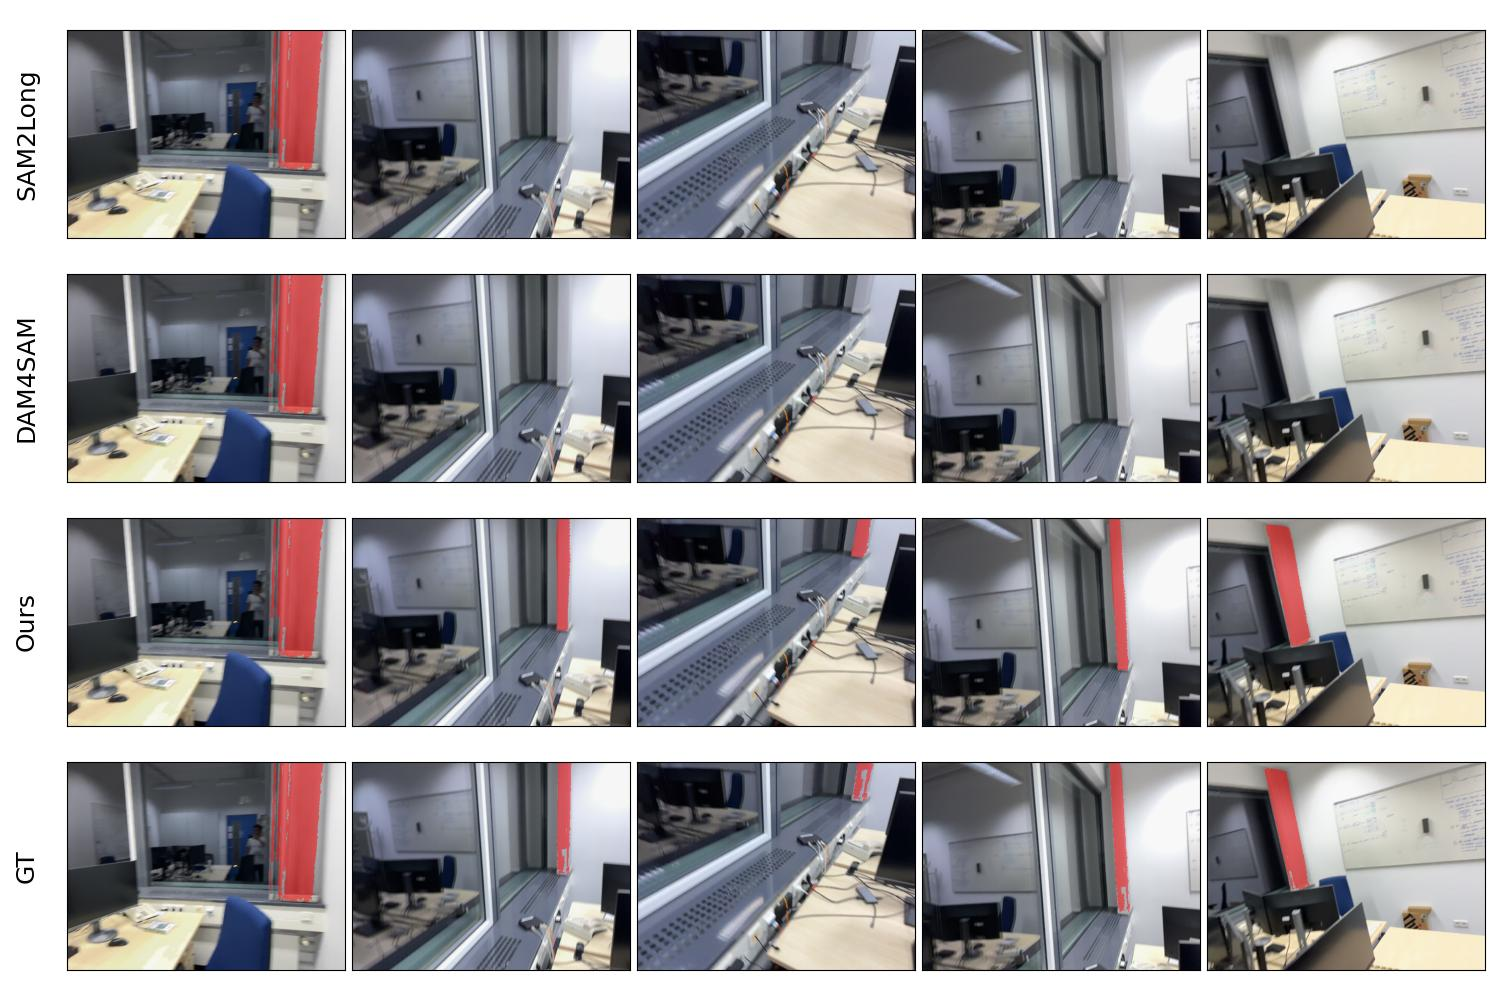
\includegraphics[width=1.0\textwidth]{figs/fig-vis/7b6477cb95/pred_masks_instance_512_45.jpg}
    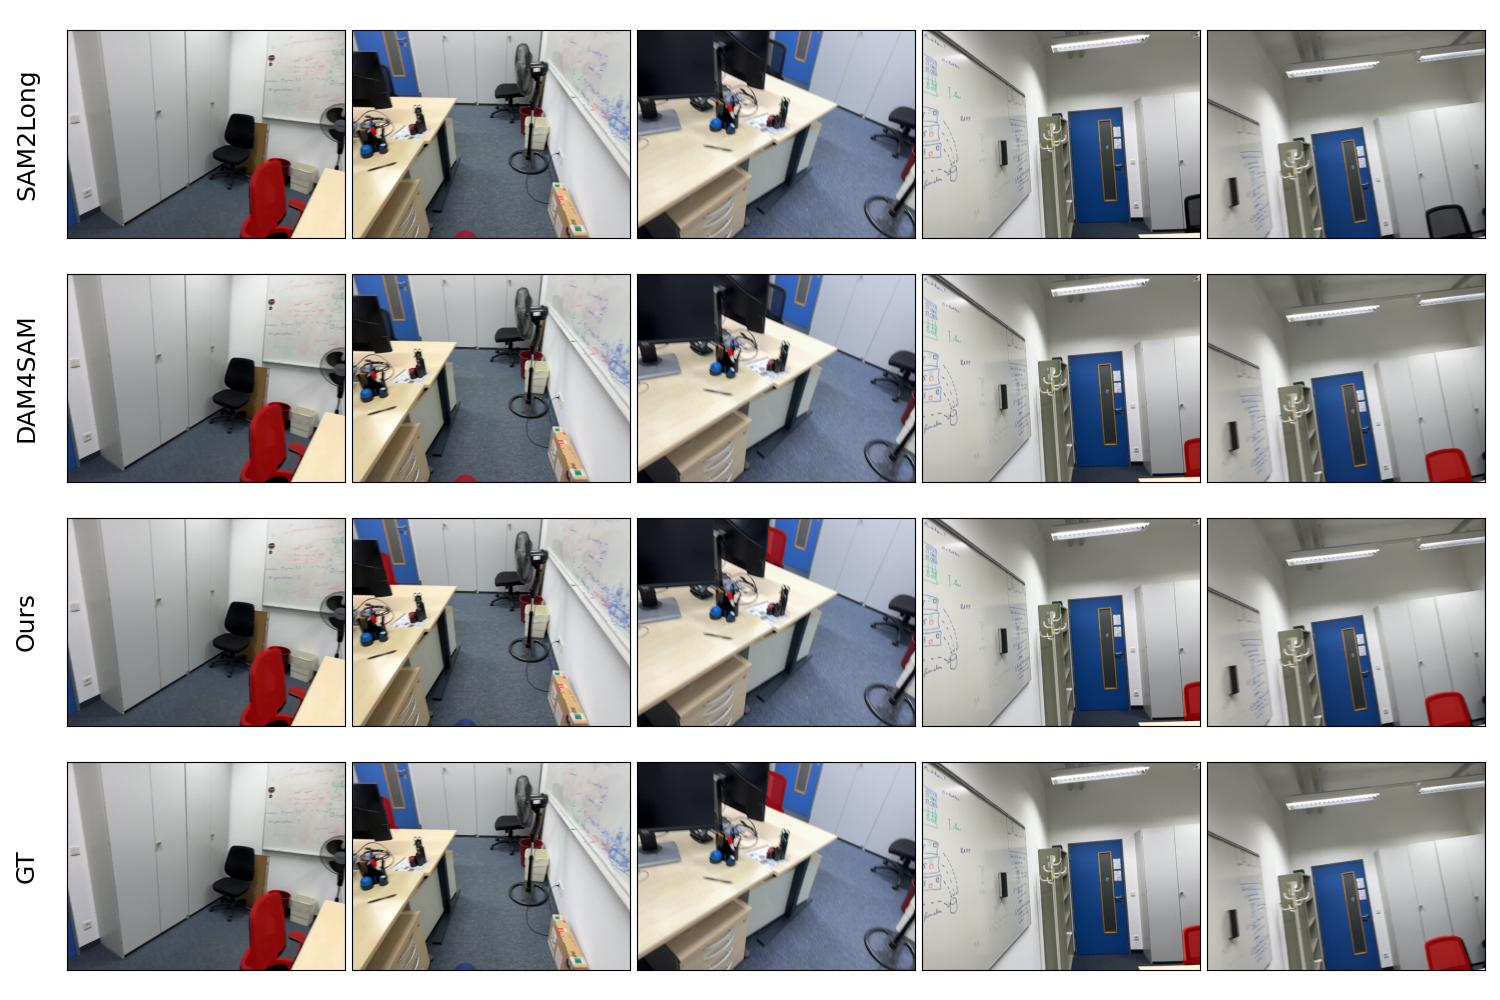
\includegraphics[width=1.0\textwidth]{figs/fig-vis/7b6477cb95/pred_masks_instance_512_53.jpg}
    \caption{
    \textbf{Visual comparison of different VOS methods}
    }
    \label{fig:vis_comp4}
\end{figure*}

\begin{figure*}[t]
    \centering
    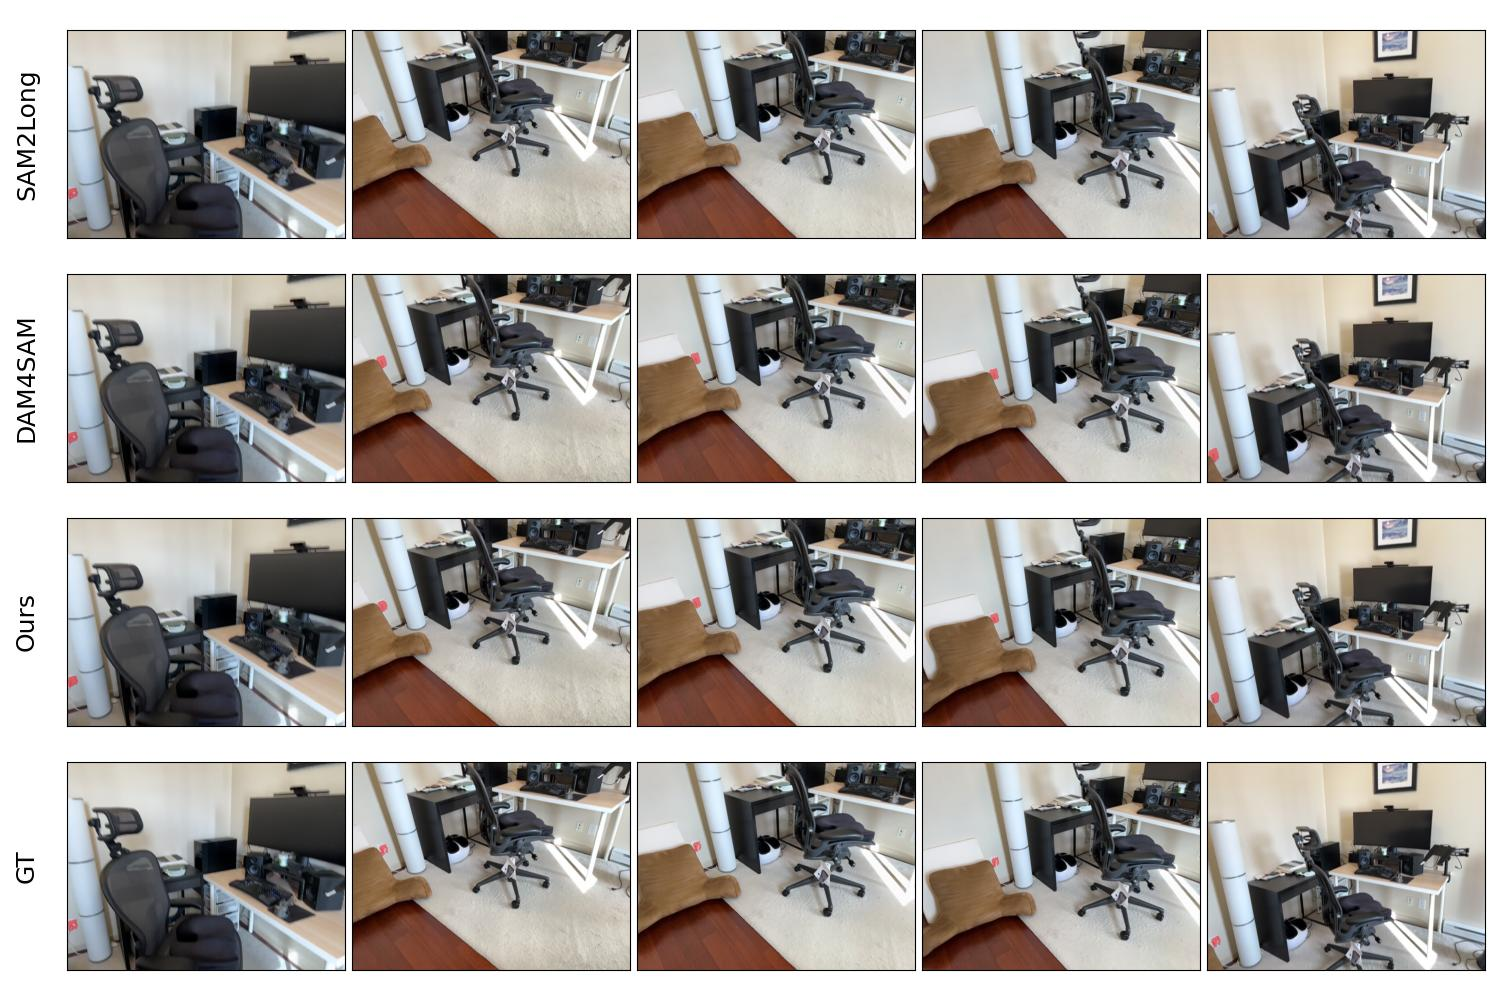
\includegraphics[width=1.0\textwidth]{figs/fig-vis/a24f64f7fb/pred_masks_instance_512_22.jpg}
    
\includegraphics[width=1.0\textwidth]{figs/fig-vis/acd95847c5/pred_masks_instance_512_10.jpg}
    \caption{
    \textbf{Visual comparison of different VOS methods}
    }
    \label{fig:vis_comp5}
\end{figure*}

\begin{figure*}[t]
    \centering
    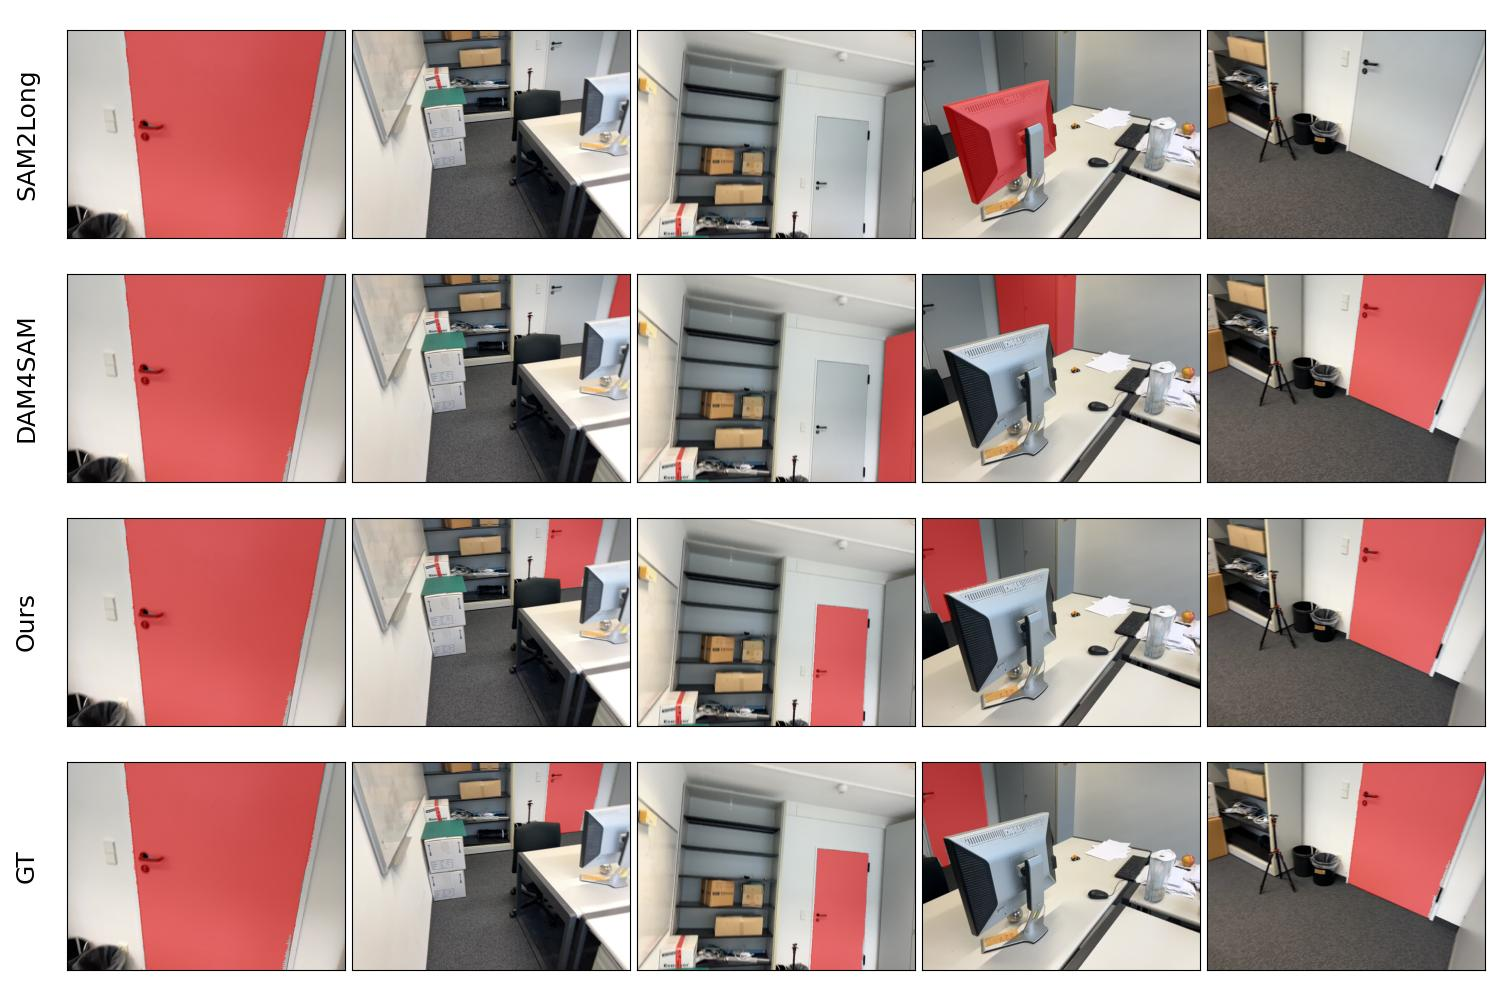
\includegraphics[width=1.0\textwidth]{figs/fig-vis/acd95847c5/pred_masks_instance_512_14.jpg}
    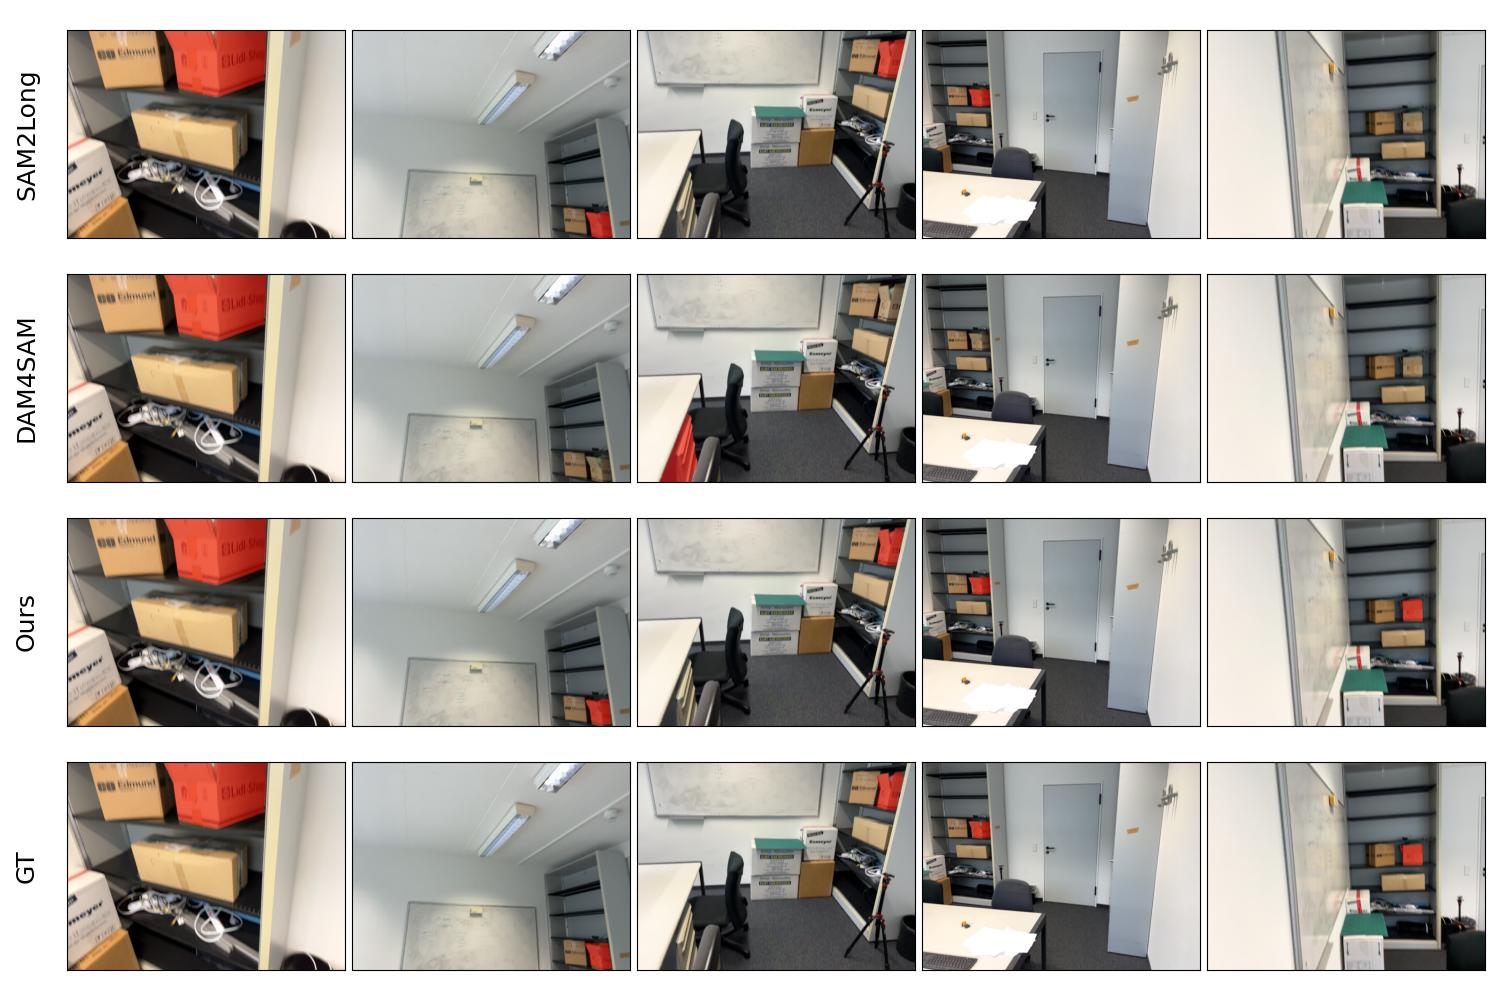
\includegraphics[width=1.0\textwidth]{figs/fig-vis/acd95847c5/pred_masks_instance_512_33.jpg}
    \caption{
    \textbf{Visual comparison of different VOS methods}
    }
    \label{fig:vis_comp6}
\end{figure*}

\begin{figure*}[t]
    \centering
    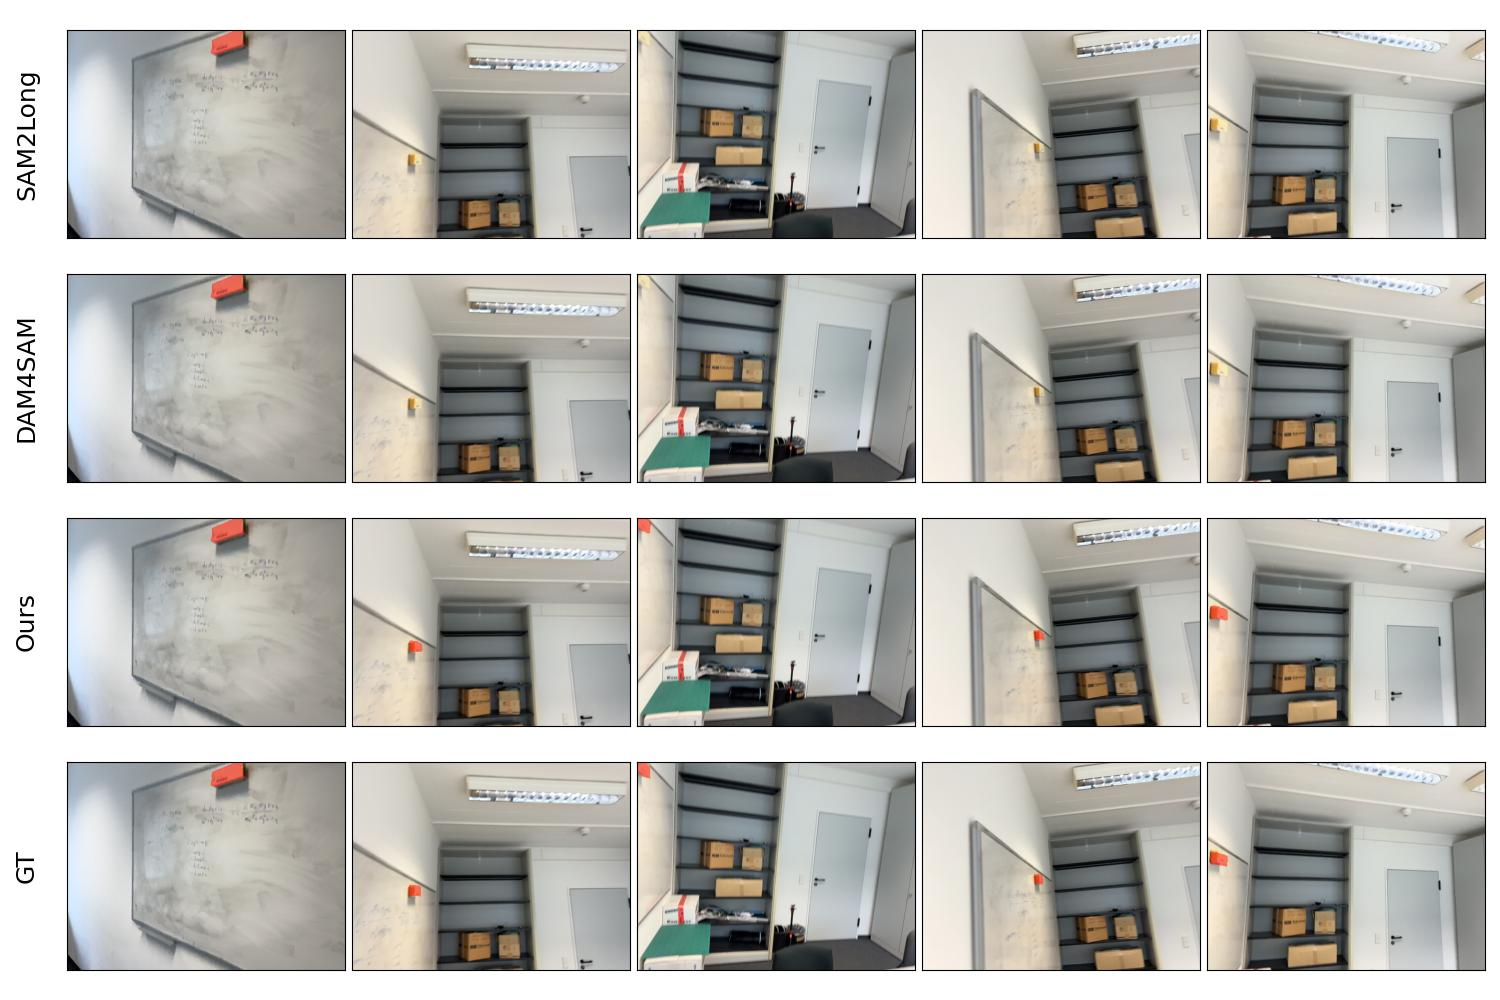
\includegraphics[width=1.0\textwidth]{figs/fig-vis/acd95847c5/pred_masks_instance_512_43.jpg}
    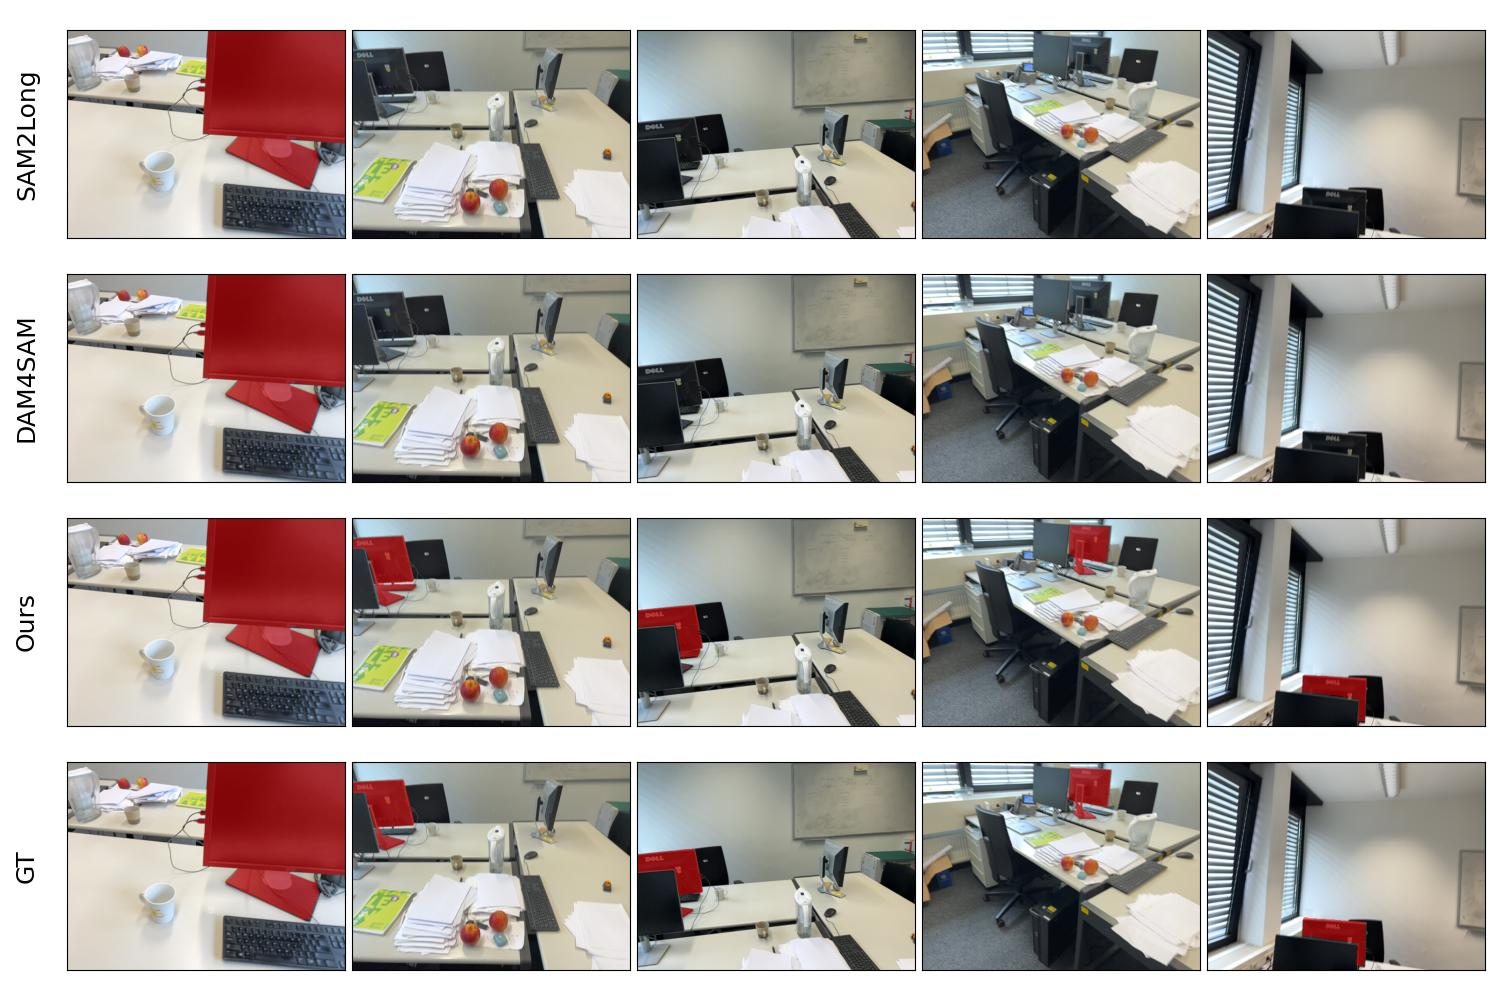
\includegraphics[width=1.0\textwidth]{figs/fig-vis/acd95847c5/pred_masks_instance_512_59.jpg}
    \caption{
    \textbf{Visual comparison of different VOS methods}
    }
    \label{fig:vis_comp7}
\end{figure*}

\section{Qualitative Comparison} \label{sec:more_qualitative}
\paragraph{Video Comparisoin}
We provide video object tracking visualization in \cref{fig:vis_comp,fig:vis_comp2,fig:vis_comp3,fig:vis_comp4,fig:vis_comp5,fig:vis_comp6,fig:vis_comp7}.
\paragraph{Class-Agnostic Instance Segmentation.}
We provide additional visual results on class-agnostic instance segmentation in~\cref{fig:visual_class}.




\begin{figure*}[ht]
\centering
\small
\setlength{\tabcolsep}{2pt}
% \renewcommand{\arraystretch}{1.0}
\resizebox{\textwidth}{!}{
\begin{tabular}{ccc}
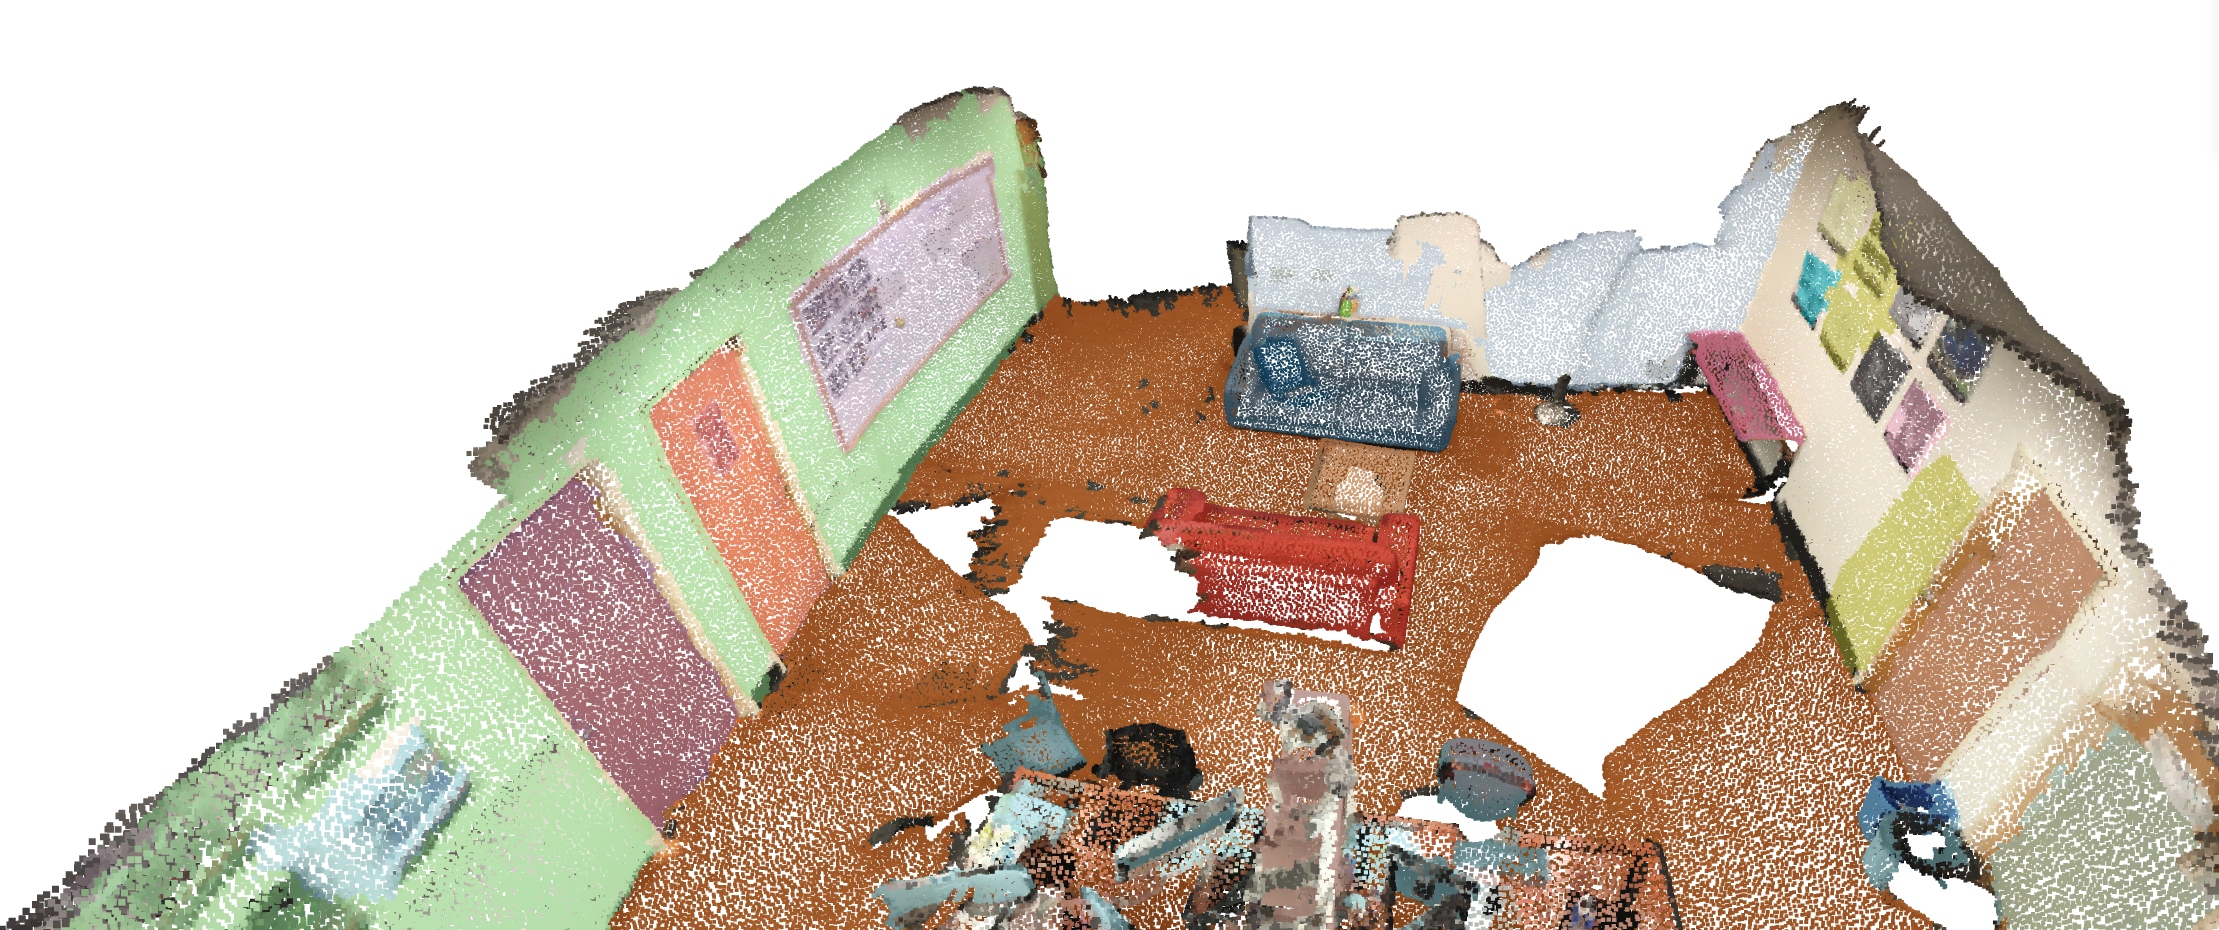
\includegraphics[width=0.33\textwidth]{figs/3D-Visual/1_1.png} & 
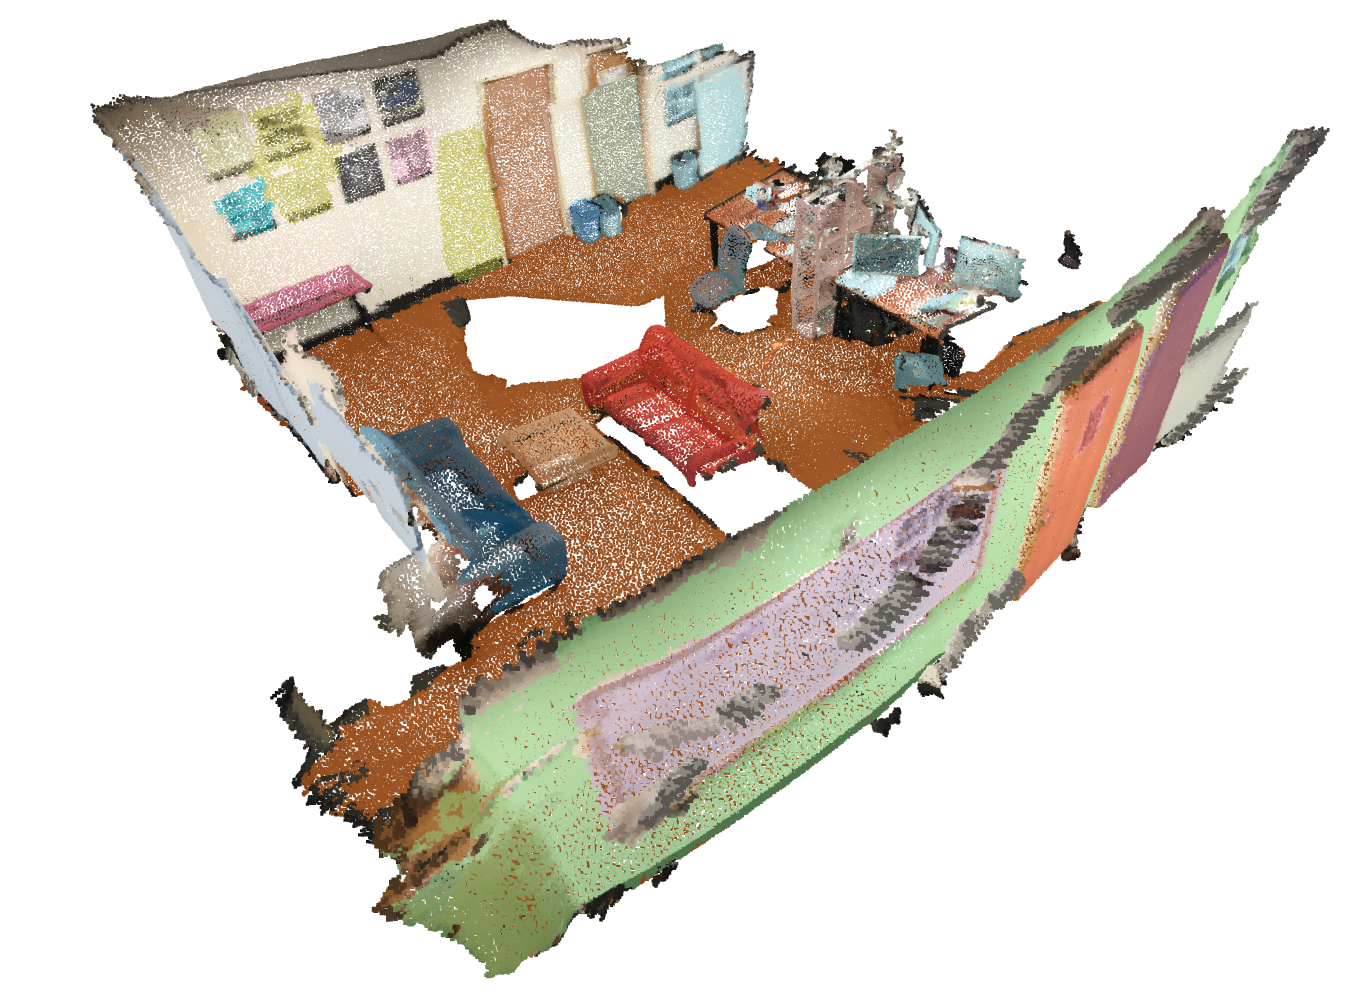
\includegraphics[width=0.33\textwidth]{figs/3D-Visual/1_2.png} & 
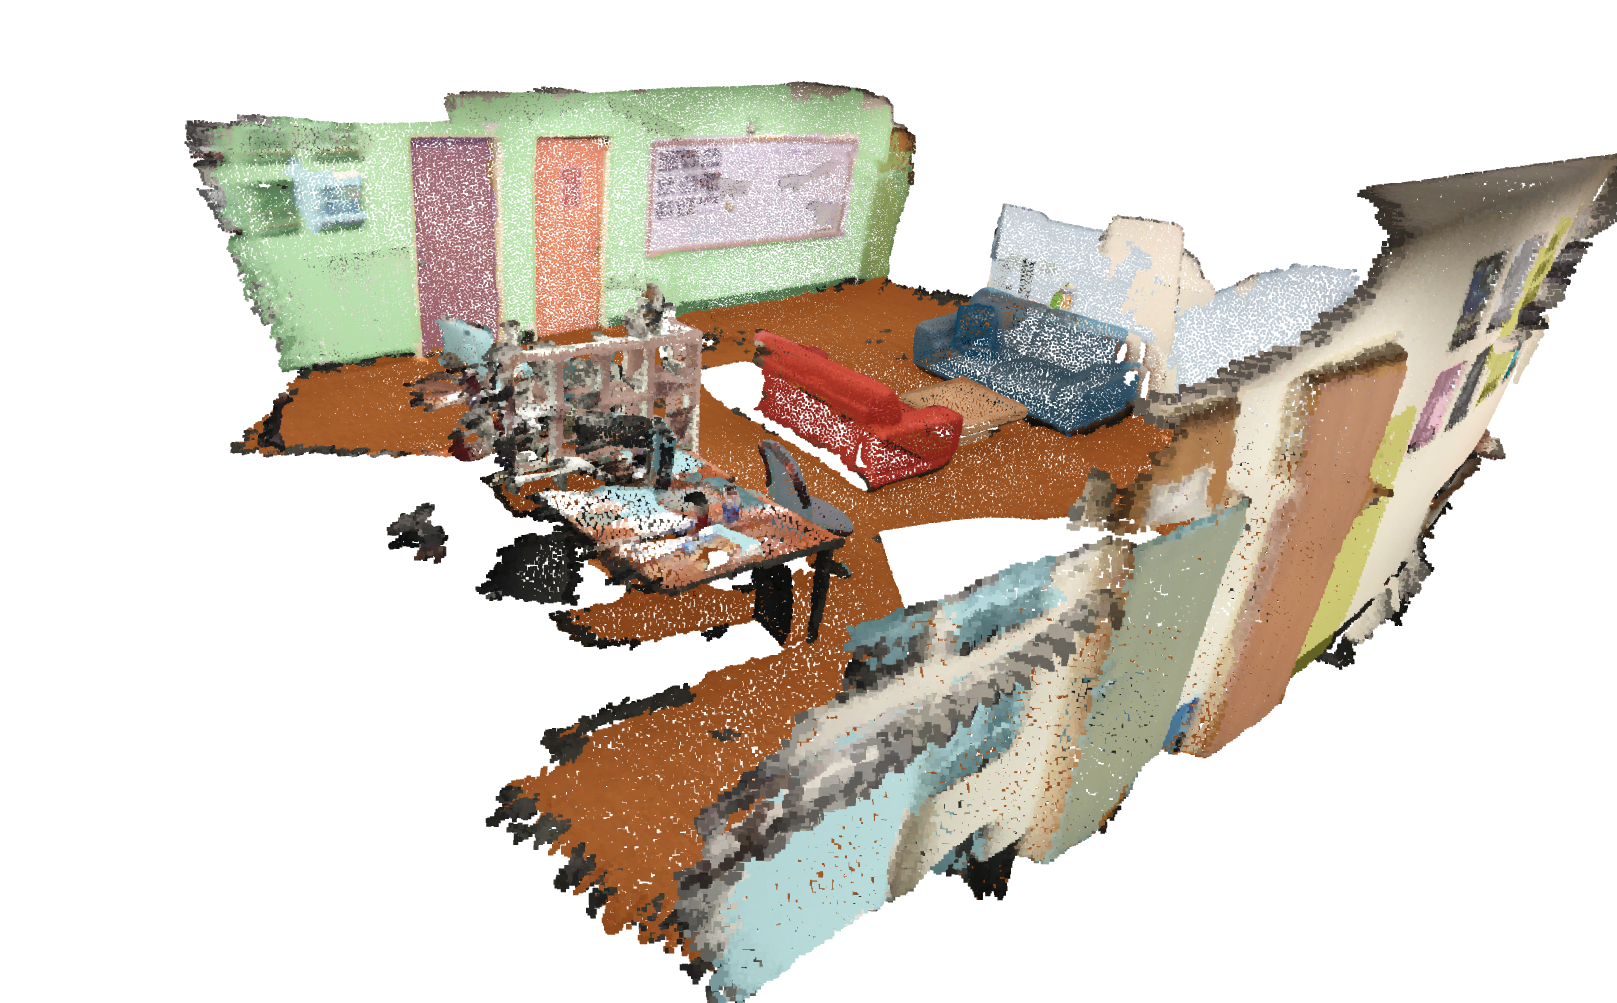
\includegraphics[width=0.33\textwidth]{figs/3D-Visual/1_3.png} \\
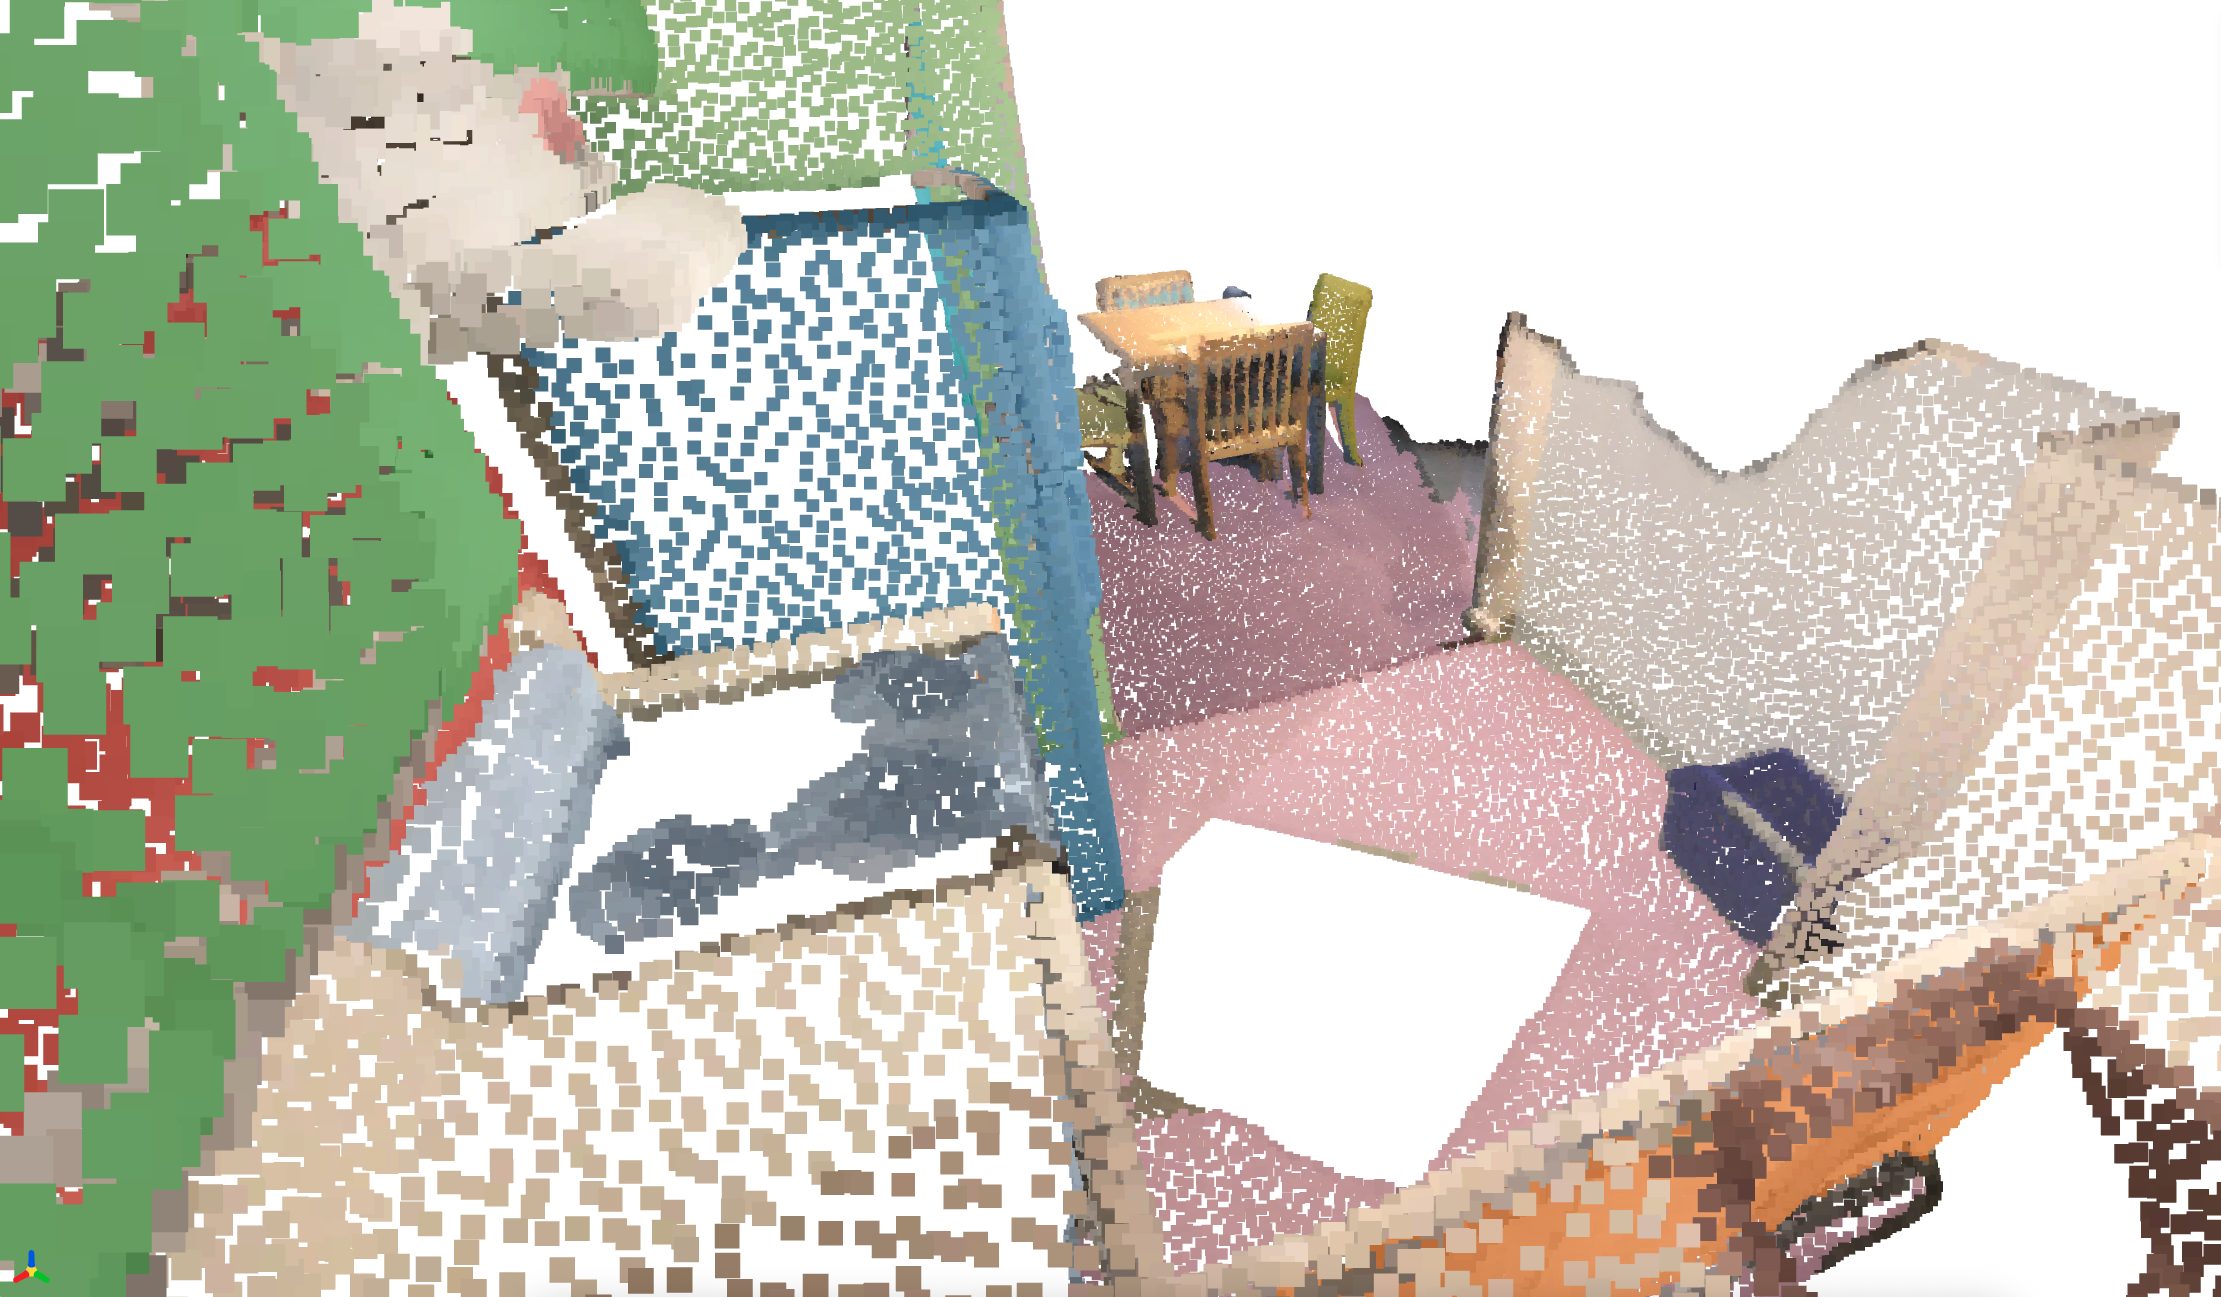
\includegraphics[width=0.33\textwidth]{figs/3D-Visual/2_1.png} & 
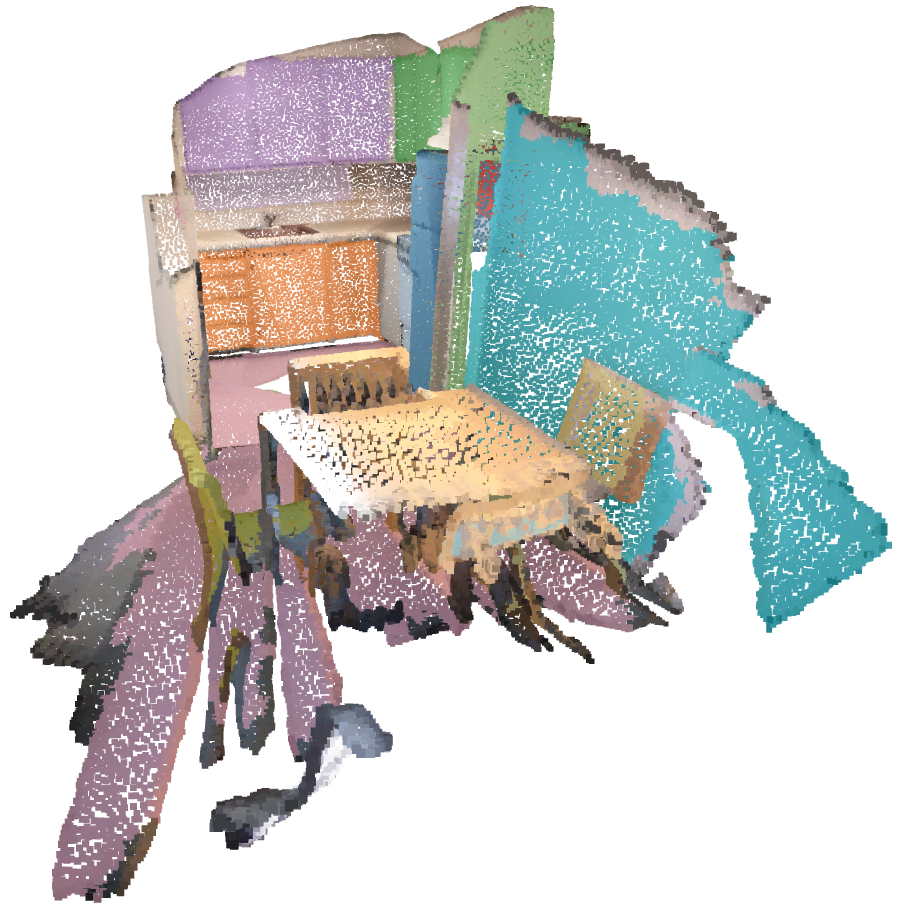
\includegraphics[width=0.33\textwidth]{figs/3D-Visual/2_2.png} & 
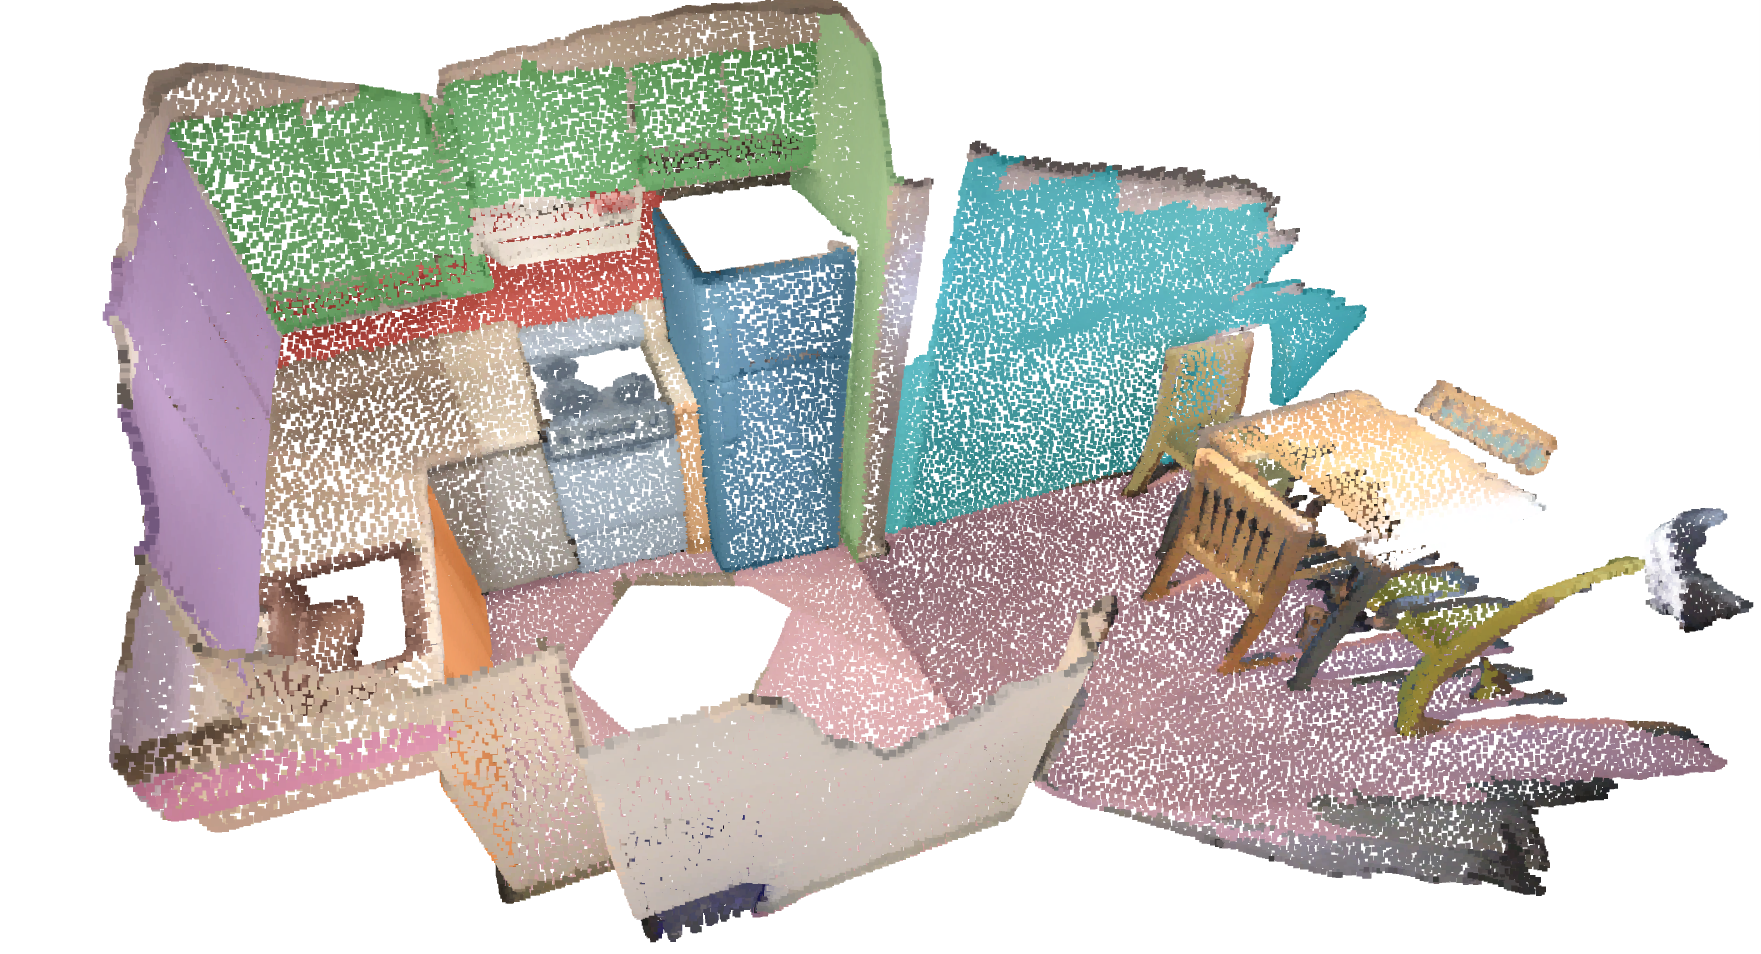
\includegraphics[width=0.33\textwidth]{figs/3D-Visual/2_3.png} \\
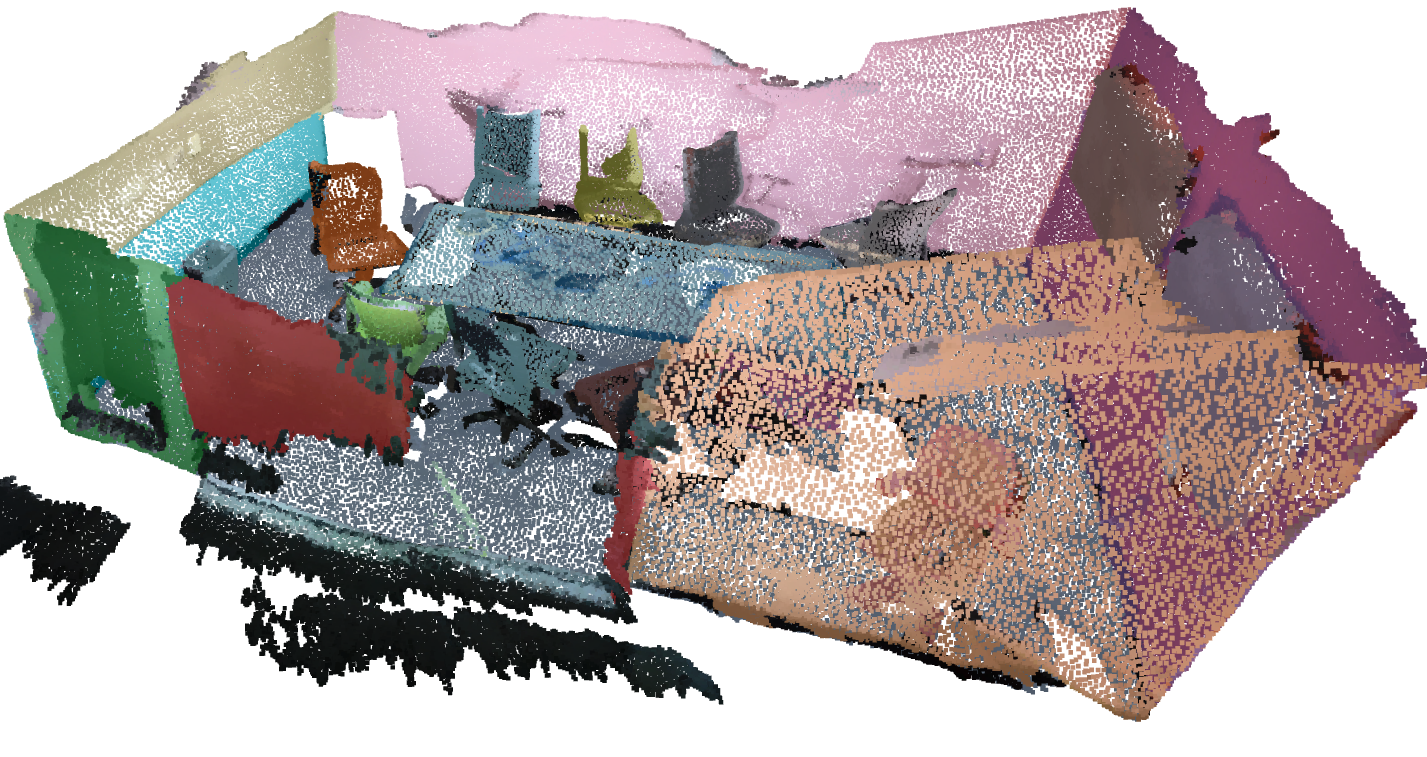
\includegraphics[width=0.33\textwidth]{figs/3D-Visual/3_1.png} & 
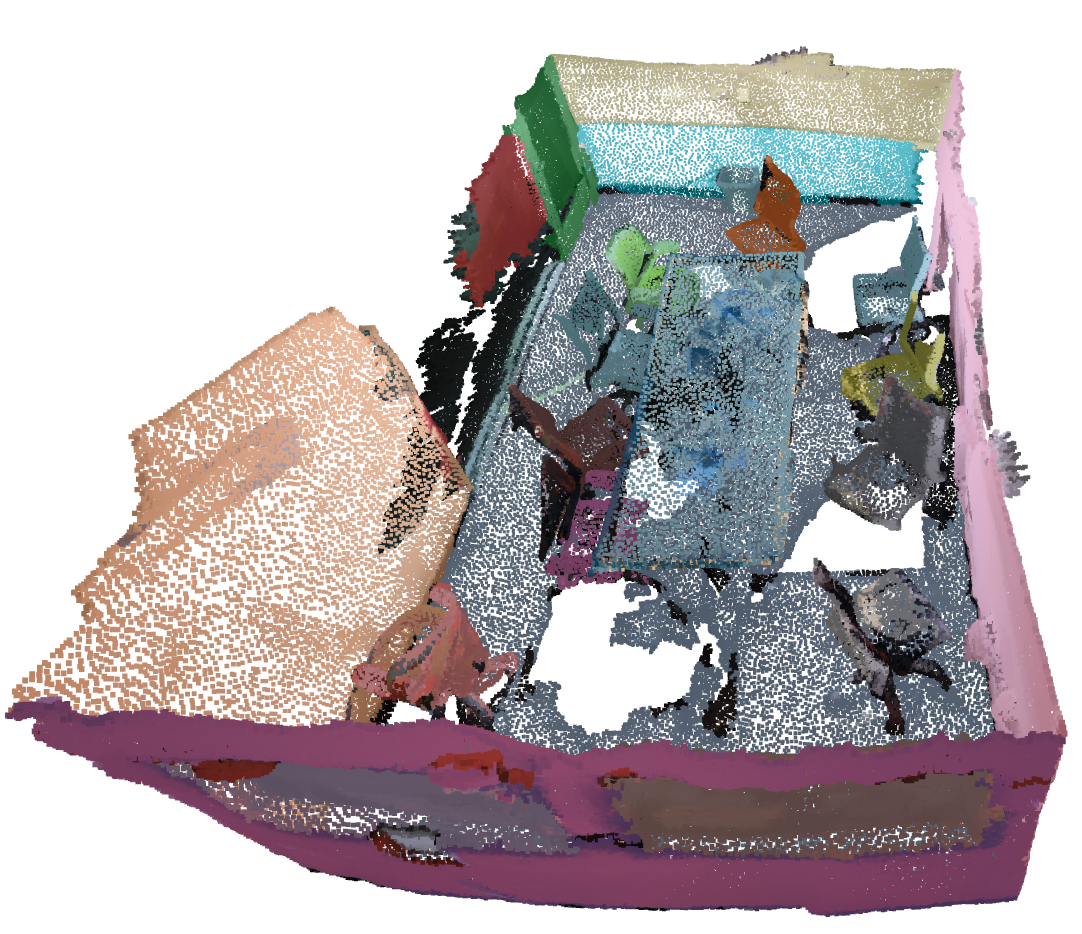
\includegraphics[width=0.33\textwidth]{figs/3D-Visual/3_2.png} & 
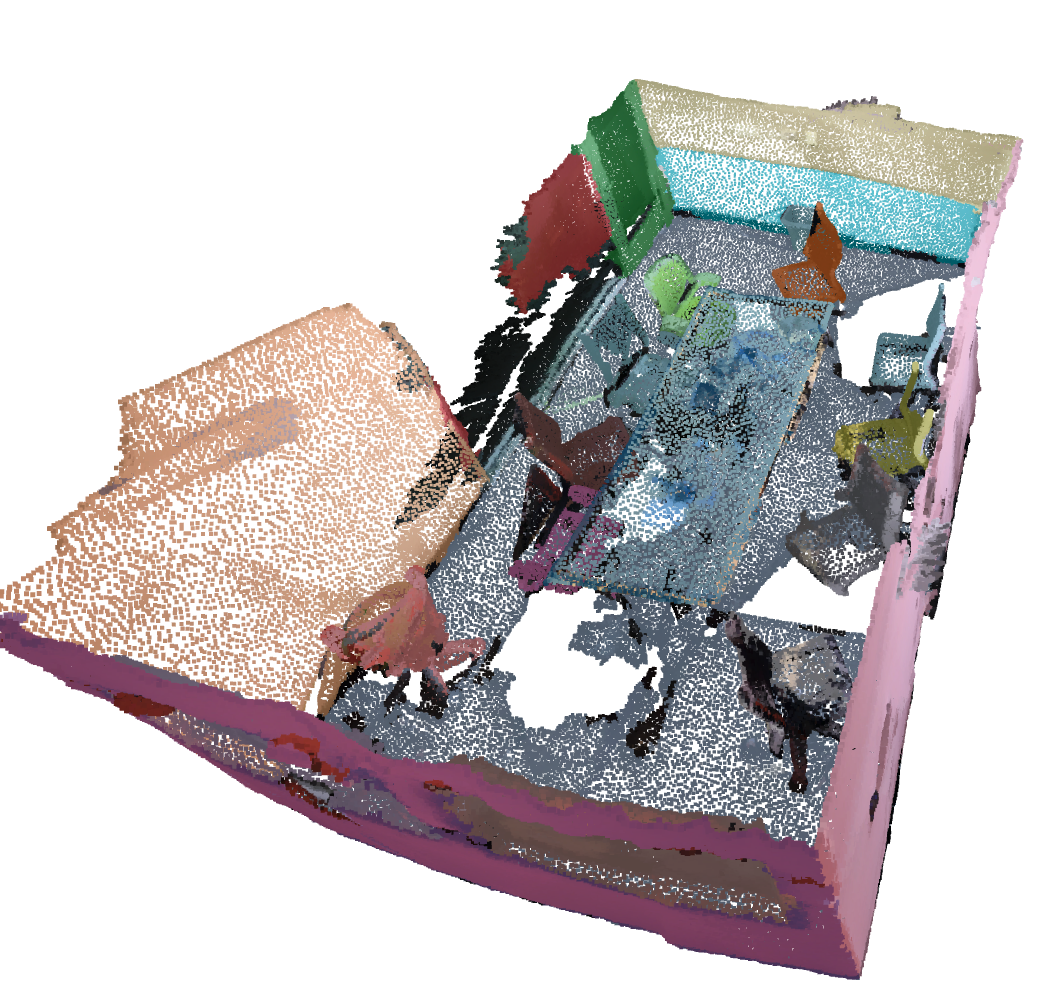
\includegraphics[width=0.33\textwidth]{figs/3D-Visual/3_3.png} \\
\end{tabular}
}
\caption{
\textbf{Visual results on class-agnostic instance segmentation.}
}
\label{fig:visual_class}
\end{figure*}


\end{document}
